\ifdefined\included
\else
\documentclass[a4paper,11pt,twoside]{StyleThese}
\usepackage{amsmath,amssymb, amsthm}             % AMS Math
\usepackage[T1]{fontenc}
\usepackage[utf8x]{inputenc}
\usepackage{babel}
\usepackage{datetime}

\usepackage{silence}

\WarningFilter{minitoc(hints)}{W0023}
\WarningFilter{minitoc(hints)}{W0028}
\WarningFilter{minitoc(hints)}{W0030}

\usepackage{lmodern}
\usepackage{tabularx}
%\usepackage{tabular}
\usepackage{multirow}
\usepackage{xspace}

\usepackage{hhline}
\usepackage[left=1.5in,right=1.3in,top=1.1in,bottom=1.1in,includefoot,includehead,headheight=13.6pt]{geometry}
\renewcommand{\baselinestretch}{1.05}

% Table of contents for each chapter

\usepackage[nottoc, notlof, notlot]{tocbibind}
\usepackage{minitoc}
\setcounter{minitocdepth}{2}
\mtcindent=15pt
% Use \minitoc where to put a table of contents

\usepackage{aecompl}

% Glossary / list of abbreviations

\usepackage[intoc]{nomencl}
\iftoggle{ThesisInEnglish}{%
\renewcommand{\nomname}{Glossary}
}{ %
\renewcommand{\nomname}{Liste des Abréviations}
}

\usepackage{etoolbox}
\renewcommand\nomgroup[1]{%
  \item[\bfseries
  \ifstrequal{#1}{A}{Number Sets}{%
  \ifstrequal{#1}{G}{Agents Beliefs and Action Models}{%
  \ifstrequal{#1}{N}{Navigation}{%
  \ifstrequal{#1}{O}{Ontology}{%
  \ifstrequal{#1}{R}{Referring Expression Generation}{%
  \ifstrequal{#1}{Z}{Controllable and Uncontrollable Agents Task Planning}{}}}}}}%
]}

\makenomenclature



% My pdf code

\usepackage{ifpdf}

\ifpdf
  \usepackage[pdftex]{graphicx}
  \DeclareGraphicsExtensions{.jpg}
  \usepackage[pagebackref,hyperindex=true]{hyperref}
  \usepackage{tikz}
  \usetikzlibrary{arrows,shapes,calc}
\else
  \usepackage{graphicx}
  \DeclareGraphicsExtensions{.ps,.eps}
  \usepackage[dvipdfm,pagebackref,hyperindex=true]{hyperref}
\fi

\graphicspath{{.}{images/}}

%% nicer backref links. NOTE: The flag ThesisInEnglish is used to define the
% language in the back references. Read more about it in These.tex

\iftoggle{ThesisInEnglish}{%
\renewcommand*{\backref}[1]{}
\renewcommand*{\backrefalt}[4]{%
\ifcase #1 %
(Not cited.)%
\or
(Cited in page~#2.)%
\else
(Cited in pages~#2.)%
\fi}
\renewcommand*{\backrefsep}{, }
\renewcommand*{\backreftwosep}{ and~}
\renewcommand*{\backreflastsep}{ and~}
}{%
\renewcommand*{\backref}[1]{}
\renewcommand*{\backrefalt}[4]{%
\ifcase #1 %
(Non cité.)%
\or
(Cité en page~#2.)%
\else
(Cité en pages~#2.)%
\fi}
\renewcommand*{\backrefsep}{, }
\renewcommand*{\backreftwosep}{ et~}
\renewcommand*{\backreflastsep}{ et~}
}

% Links in pdf
\usepackage{color}
\definecolor{linkcol}{rgb}{0,0,0.4} 
\definecolor{citecol}{rgb}{0.5,0,0} 
\definecolor{linkcol}{rgb}{0,0,0} 
\definecolor{citecol}{rgb}{0,0,0}
% Change this to change the informations included in the pdf file

\hypersetup
{
bookmarksopen=true,
pdftitle="Planning For Both Robot and Human: Anticipating and Accompanying Human Decisions",
pdfauthor="Guilhem BUISAN", %auteur du document
pdfsubject="Thèse", %sujet du document
%pdftoolbar=false, %barre d'outils non visible
pdfmenubar=true, %barre de menu visible
pdfhighlight=/O, %effet d'un clic sur un lien hypertexte
colorlinks=true, %couleurs sur les liens hypertextes
pdfpagemode=None, %aucun mode de page
pdfpagelayout=SinglePage, %ouverture en simple page
pdffitwindow=true, %pages ouvertes entierement dans toute la fenetre
linkcolor=linkcol, %couleur des liens hypertextes internes
citecolor=citecol, %couleur des liens pour les citations
urlcolor=linkcol %couleur des liens pour les url
}

% definitions.
% -------------------

\setcounter{secnumdepth}{3}
\setcounter{tocdepth}{2}

% Some useful commands and shortcut for maths:  partial derivative and stuff

\newcommand{\pd}[2]{\frac{\partial #1}{\partial #2}}
\def\abs{\operatorname{abs}}
\def\argmax{\operatornamewithlimits{arg\,max}}
\def\argmin{\operatornamewithlimits{arg\,min}}
\def\diag{\operatorname{Diag}}
\newcommand{\eqRef}[1]{(\ref{#1})}

\usepackage{rotating}                    % Sideways of figures & tables
%\usepackage{bibunits}
%\usepackage[sectionbib]{chapterbib}          % Cross-reference package (Natural BiB)
%\usepackage{natbib}                  % Put References at the end of each chapter
                                         % Do not put 'sectionbib' option here.
                                         % Sectionbib option in 'natbib' will do.
\usepackage{fancyhdr}                    % Fancy Header and Footer

% \usepackage{txfonts}                     % Public Times New Roman text & math font
  
%%% Fancy Header %%%%%%%%%%%%%%%%%%%%%%%%%%%%%%%%%%%%%%%%%%%%%%%%%%%%%%%%%%%%%%%%%%
% Fancy Header Style Options

\pagestyle{fancy}                       % Sets fancy header and footer
\fancyfoot{}                            % Delete current footer settings

%\renewcommand{\chaptermark}[1]{         % Lower Case Chapter marker style
%  \markboth{\chaptername\ \thechapter.\ #1}}{}} %

%\renewcommand{\sectionmark}[1]{         % Lower case Section marker style
%  \markright{\thesection.\ #1}}         %

\fancyhead[LE,RO]{\bfseries\thepage}    % Page number (boldface) in left on even
% pages and right on odd pages
\fancyhead[RE]{\bfseries\nouppercase{\leftmark}}      % Chapter in the right on even pages
\fancyhead[LO]{\bfseries\nouppercase{\rightmark}}     % Section in the left on odd pages

\let\headruleORIG\headrule
\renewcommand{\headrule}{\color{black} \headruleORIG}
\renewcommand{\headrulewidth}{1.0pt}
\usepackage{colortbl}
\arrayrulecolor{black}

\fancypagestyle{plain}{
  \fancyhead{}
  \fancyfoot{}
  \renewcommand{\headrulewidth}{0pt}
}

%\usepackage{MyAlgorithm}
%\usepackage[noend]{MyAlgorithmic}
\usepackage{algorithm}
\usepackage[noend]{algpseudocode}
\usepackage{comment}
\usepackage[ED=EDSYS-Robo, Ets=INSA]{tlsflyleaf}
%%% Clear Header %%%%%%%%%%%%%%%%%%%%%%%%%%%%%%%%%%%%%%%%%%%%%%%%%%%%%%%%%%%%%%%%%%
% Clear Header Style on the Last Empty Odd pages
\makeatletter

\def\cleardoublepage{\clearpage\if@twoside \ifodd\c@page\else%
  \hbox{}%
  \thispagestyle{empty}%              % Empty header styles
  \newpage%
  \if@twocolumn\hbox{}\newpage\fi\fi\fi}

\makeatother
 
%%%%%%%%%%%%%%%%%%%%%%%%%%%%%%%%%%%%%%%%%%%%%%%%%%%%%%%%%%%%%%%%%%%%%%%%%%%%%%% 
% Prints your review date and 'Draft Version' (From Josullvn, CS, CMU)
\newcommand{\reviewtimetoday}[2]{\special{!userdict begin
    /bop-hook{gsave 20 710 translate 45 rotate 0.8 setgray
      /Times-Roman findfont 12 scalefont setfont 0 0   moveto (#1) show
      0 -12 moveto (#2) show grestore}def end}}
% You can turn on or off this option.
% \reviewtimetoday{\today}{Draft Version}
%%%%%%%%%%%%%%%%%%%%%%%%%%%%%%%%%%%%%%%%%%%%%%%%%%%%%%%%%%%%%%%%%%%%%%%%%%%%%%% 

\newenvironment{maxime}[1]
{
\vspace*{0cm}
\hfill
\begin{minipage}{0.5\textwidth}%
%\rule[0.5ex]{\textwidth}{0.1mm}\\%
\hrulefill $\:$ {\bf #1}\\
%\vspace*{-0.25cm}
\it 
}%
{%

\hrulefill
\vspace*{0.5cm}%
\end{minipage}
}

\let\minitocORIG\minitoc
\renewcommand{\minitoc}{\minitocORIG \vspace{1.5em}}

\usepackage{multirow}
%\usepackage{slashbox}

\newenvironment{bulletList}%
{ \begin{list}%
	{$\bullet$}%
	{\setlength{\labelwidth}{25pt}%
	 \setlength{\leftmargin}{30pt}%
	 \setlength{\itemsep}{\parsep}}}%
{ \end{list} }

\theoremstyle{definition}
\newtheorem{definition}{Definition}
\renewcommand{\epsilon}{\varepsilon}

% centered page environment

\newenvironment{vcenterpage}
{\newpage\vspace*{\fill}\thispagestyle{empty}\renewcommand{\headrulewidth}{0pt}}
{\vspace*{\fill}}

\usepackage{tablefootnote}

\theoremstyle{plain}
\newtheorem{constraint}{Constraint}[section]

\algnewcommand\algorithmicforeach{\textbf{for each}}
\algnewcommand\algorithmicin{\textbf{in}}
\algdef{S}[FOR]{ForEach}[2]{\algorithmicforeach\ #1\ \algorithmicin\ #2\ \algorithmicdo}

\usepackage{listings}
\lstdefinestyle{customPlan}{
  language=C,
  commentstyle=\itshape\color{green!25!black},
}
\usepackage{pdfpages}

\sloppy
\begin{document}
\setcounter{chapter}{2} %% Numéro du chapitre précédent ;)
\dominitoc
\faketableofcontents
\fi

\chapter{Evaluating Communications Feasibility and Cost During Human-Aware Task Planning}
\label{chapter:comm}
\chaptermark{Determining Communications During Planning}
\minitoc

\section{Introduction and Example}
In the previous chapter, we showed interactions are more efficient and satisfactory if the robot considers the plan of the human in its own course of action. Not only it allows at least to ensure that the task is feasible for both agents (provided the models are correct enough) but also to perform coordination smoothers or other communication actions.

In this chapter, we alleviate from the inherently ephemeral nature of interaction in geometrical navigation planning to further study at symbolic level the planning of communication actions in plans involving multiple agents. Communication between the agents can be made in two ways. Either some of the planned actions convey information but have another main effect or they are dedicated communication actions having no other (intended) effect. The former is linked to predictability and legibility of motion as formalized by Dragan \cite{dragan_legibility_2013}. Moreover, we explored part of it in the previous chapter, as we were using a navigation scheme planning for both the human and the robot to add coordination smoothers to the robot trajectory. The latter is what we will be discussed in this chapter. Especially, we will focus on one type of explicit communication, being verbally designating an object, a problem called referring expression generation.

This raises two questions:
\begin{itemize}
\item \textbf{How to determine the pertinence and the cost of a communication action in task planning?}
\item \textbf{When must the robot perform a communication action?}
\end{itemize}
These questions can boil down to \textit{what} and \textit{when} to communicate \cite{mavridis2015review}. While determining \textit{when} to insert the verbal communication actions in a human robot joint plan is the goal of a task planner, why resolving the \textit{what} during task planning may not be obvious. First, some communications are more costly than others. We use the cost of a communication action to represent the difficulty to understand it when received by the human and the difficulty to generate it when emitted by the human. In some contexts designating an object among others can be hard. Then, in some cases the communication is not feasible not because of a physical inability (\textit{e.g.}~the robot and the human being far apart) but because the content cannot be resolved. Thus, determining the \textit{what} will impact the \textit{when}.

Similarly, the content of a communication will not be the same depending on when it is done. The evolving world state along the plan execution will change the way to refer to an object. Some other objects can be added or removed as the task progresses. Some communications will be crucial for the plan at a certain point while others appearing to be needed will reveal to be optional. Thus, we also need to the \textit{when} to communicate to know \textit{what} will be communicated.

\subsection{Example}
\begin{figure}[hbtp]
\centering
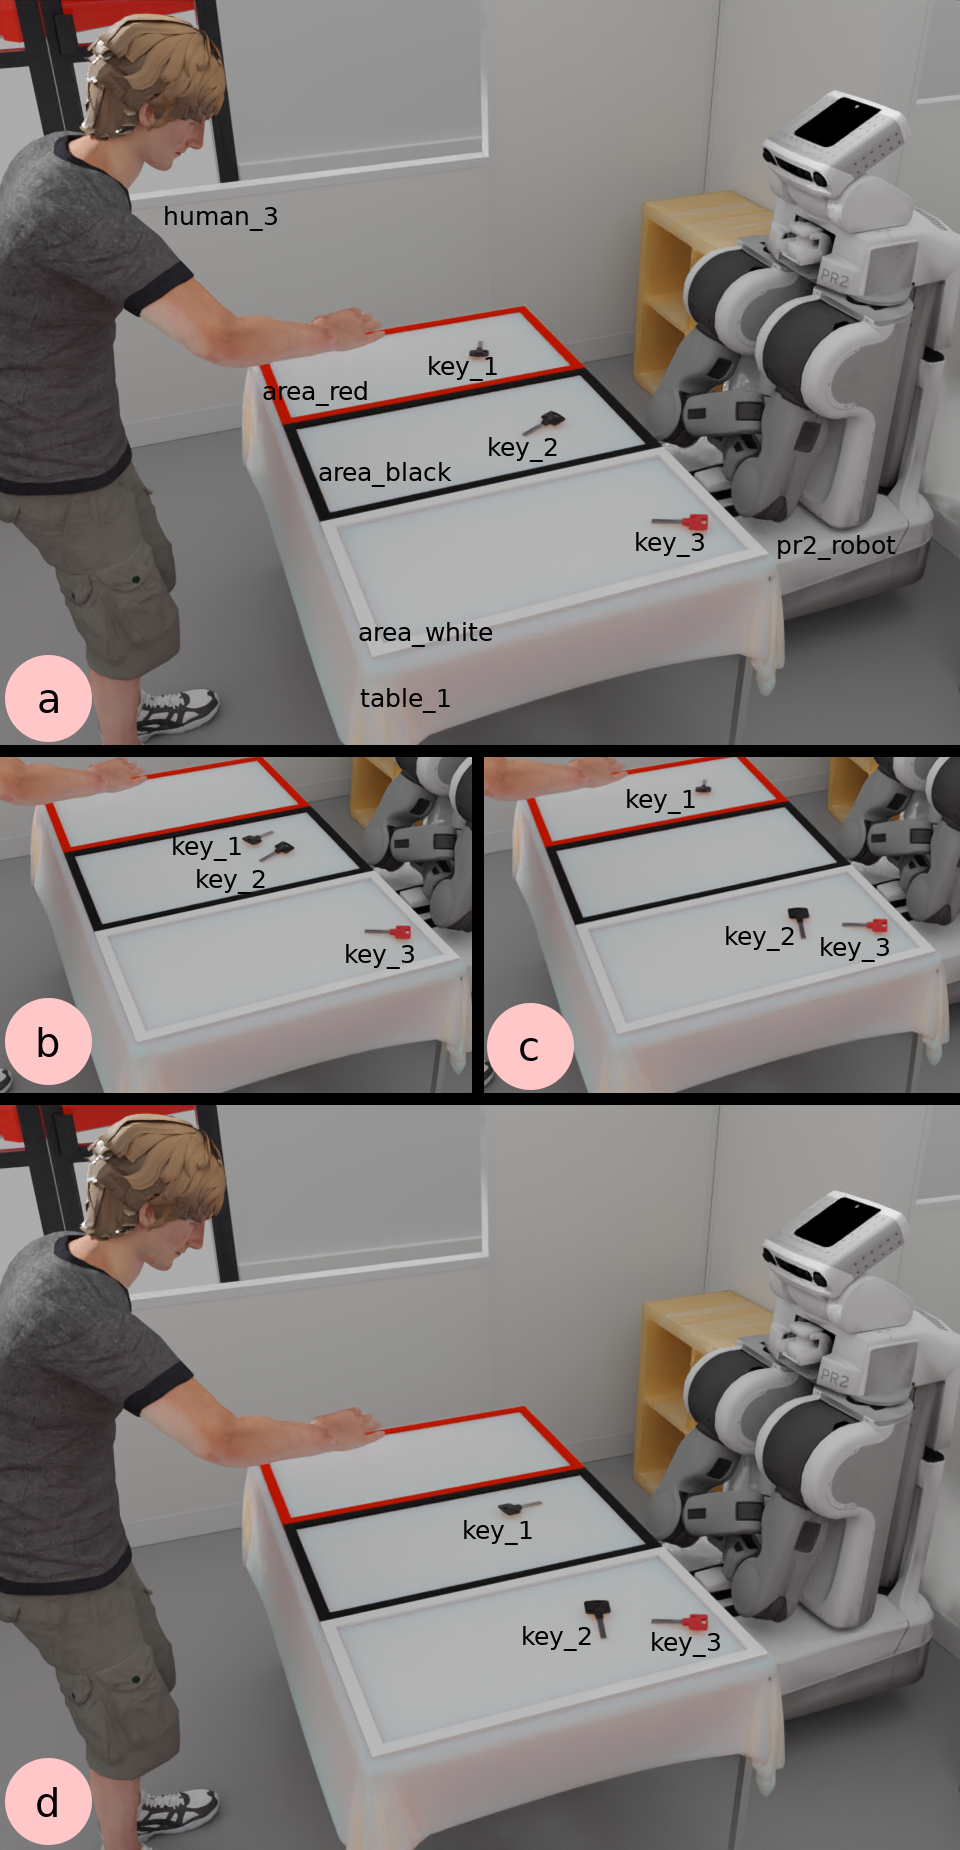
\includegraphics[scale=0.27]{figures/chapter3/Chap3illustrative.png}
\caption{A simple example where the robot and the human must cooperate to sort keys. Only the robot knows the goal state (d). It has to communicate to the human, one at a time, which key to grab and where to put them.  From the initial state (a) the robot can either communicate to move \texttt{key\_1} leading to state (b) or to move \texttt{key\_2} leading to state (c). In (b) the situation is locked as \texttt{key\_1} and \texttt{key\_2} are identical. In (c) the robot can communicate to move \texttt{key\_1} to reach the goal state (d).}
\label{fig:chap3keys}
\end{figure}

In order to clarify the problem and illustrate this chapter contents, let us take the situation depicted in Figure~\ref{fig:chap3keys}(a). In this situation, a human and his robot partner are trying to organize different car keys. The areas represent which car a key opens, and multiple keys can open the same car. The keys are distributed randomly at first. The human does not know which key opens which car, but the robot does thanks to an integrated RFID system. The robot, for which the keys are too small to manipulate, has then to give instructions to the human for where to put the keys. The keys are only distinguishable by the human through their colors and the color of the area they sit in, and he can manipulate only one at a time. Besides, the robot cannot use ``left'' or ``right'' indications nor use past human actions.
The goal, known only by the robot, is depicted in Figure~\ref{fig:chap3keys}(d). The robot has multiple ways to designate the keys and the areas to the human, it can either point to them or verbally designate them. While pointing can be straightforward, it becomes less and less accurate as the distance increases, and impossible if the perspective difference between the agents is too big. Thus, we propose to make the robot able to verbally designate the different entities in the environment.
Whatever the communication modality, to move the keys from the initial state (Figure~\ref{fig:chap3keys}(a)) to the goal state (Figure~\ref{fig:chap3keys}(d)), the robot has two main options. First, it can ask the human to move \verb'key_1' into the black area (Figure~\ref{fig:chap3keys}(b)). However, with the constraints we defined before, the robot would have no way of telling the human to take \verb'key_2', as the human cannot distinguish them anymore, as both \verb'key_1' and \verb'key_2' are the same color and in the same area. The second solution of making the human move \verb'key_2' first, provides more options to the robot, as \verb'key_1' is still verbally designable in the new situation (Figure~\ref{fig:chap3keys}(c)).

With this example, we showed that computing communication content during task planning is important as it can impact the choice of communication modalities, the plan cost, or even the feasibility of the plan (\textit{e.g.}~if the robot cannot point, the first option would not be feasible). This raises two issues we treat in this chapter: how to efficiently estimate the feasibility and cost of communication and how to use this knowledge during task planning.

To do so, we propose to use a multi-modal planning approach, where a \textit{domain-independent} task planner delegates, for specific verbal communication actions, to a \textit{domain-specific} planner designed to resolve the content of referring expressions. While the former will provide specific requests along with the context and the planned world state in which the communication is made, the latter will indicate not only the feasibility of the communication in the specific world state, but will also return a cost representing the estimated complexity to interpret this referring expression, allowing for balancing between multiple plans. This approach is greatly inspired by combined task and motion planning schemes \cite{gharbi2015combining} where a task planner uses a geometrical planner to refine motion action at the task planning level, allowing to find more precise plans.

\subsection{References and Acknowledgments}
A large part of this chapter is excerpted from our work, published for the RO-MAN 2020 conference \cite{buisan2020efficient} and for the ICSR 2020 conference \cite{buisan2020human}. However, in this manuscript, the examples are more detailed and the approaches are explained more in depth. Besides, we hope that the link between these two works appears more clearly.

The work presented in this chapter has been done in close collaboration with Guillaume Sarthou, who is working on knowledge bases for \acrshort{hri} and their uses.

\medskip

First, we review the literature concerning referring expression generation and communication actions in task planning. Then we present a novel approach for referring expression generation, which runs on ontologies and is both efficient and suitable for human robot interaction scenarios. We then show how such a planner resolving the content of referring expressions can be included in task planning allowing for precise estimation of this communication type feasibility and cost at task planning level. This approach shows the use of hybrid planning (a domain-independent planner delegating to a domain-specific planner) for \acrshort{hri}, where the domain-independent planner plans for both agents and the domain-specific planner needs the estimation of the human beliefs from the first planner.

\section{Related Work}
Estimating the content of some communication at the task planning level is needed to generate feasible and optimal plans. Indeed, some communication actions are known to be necessary already while elaborating a plan, but might not be feasible. We explore this problem by focusing on a specific communication type: the referring expression. Indeed, verbally referring to an object is challenging for several reasons. 

First, it heavily depends on the current situation. If the object to refer to is among multiple identical objects, the communication may be impossible. Similarly, the communication is getting easier the more heterogeneous the nearby objects are and the fewer objects there are. 

Then, referring to an object to another agent requires to take their perspective or to estimate their beliefs. Indeed, to refer to a key in Figure~\ref{fig:chap3keys}, the robot must estimate that the human knows the color of the keys and knows in which area they are placed.

Finally, generating a referring expression must be done in a specific context that needs to be defined. In the example depicted in Figure~\ref{fig:chap3keys}, they may be other keys in the building that the human is aware of (and that the robot knows the human is aware of) but in the context of this task, they are not considered by the human as being potentially referred to.

However, this type of communication is explicit and can accurately be represented as an action in a task planning domain. Moreover, a referring communication action may need multiple expression generation. For instance, in Figure~\ref{fig:chap3keys}(a) we can represent a robot action asking the human to move \verb'key_2' in \verb'area_white' in one sentence. This sentence would need two referring expressions: one for \verb'key_2' and one for \verb'area_white'. Thus, estimating the feasibility and cost of this action would require multiple calls to the referring expression generation planner.

In this section, we will firstly review how a robot can autonomously verbally designate an object to a hearer. This problem is called the \acrfull{reg} problem.
Then, we will review several task planning approaches allowing to account for communication actions.

\subsection{Referring Expression Generation}
As defined by Reiter and Dale, \acrfull{reg} ``\textit{is concerned with how we produce a description of an entity that enables the hearer to identify that entity in a given context}'' \cite{reiter1997building}. An intuition about what a well constructed \acrfull{re} is given by the Grice's maxims \cite{grice1975logic}. These maxims aim at defining principles for smooth cooperative activities (including verbal designation communication). They fall into four categories:
\begin{itemize}
\item \textit{Quantity}: The communication should be as informative as required but not more.
\item \textit{Quality}: The communication should be as true as possible. The sender should not communicate information that they consider false or unsure.
\item \textit{Relation}: The communication should be relevant in the current context. This is especially important when performing a collaborative task, where the world state is constantly changing and the relevance of a communication can quickly change.
\item \textit{Manner}: The communication should be unambiguous and brief.
\end{itemize}

The \acrshort{reg} problem is actually composed of two parts: the content determination --- aiming at deciding which attributes (and relations) to use --- and the linguistic realization --- refining the attributes of the content into verbalizable/writable words \cite{krahmer2012computational}. In this thesis, we will only consider the content determination, as we assume that the linguistic realization will not have any impact on the feasibility and the cost of the referring communication action once the content of the RE has been decided.

To our knowledge, the first \acrshort{reg} formulation and algorithm was coined by Dale and used a depth-first search over a knowledge base being a key-value tree representing the attributes of objects \cite{dale1989cooking}. However, this approach leads to over-specified referring expressions, containing redundant information and thus violating the maxim of quantity. On the example depicted in Figure~\ref{fig:chap3keys}(a), to refer to the \verb'key_1', provided with the right knowledge base, this approach would have led to a set of relations which could have been verbalized as ``the black key in the red area on the table'' while only ``the key in the red area'' would have sufficed in this context. This defect was corrected in a subsequent contribution with the \textit{Full Brevity} algorithm \cite{dale1992generating}, always generating the shortest referring expression, but at the cost of an exhaustive search. Besides, to be as relevant as possible, the attributes of the referred object to be included in the \acrshort{re} should be chosen carefully. Indeed, not all the attributes are equally understandable by the hearer, the color or the shape for example will often be quicker to apprehend than spatial relation. The Incremental Algorithm is the first approach tackling this issue \cite{dale1995computational}. By taking as input a preference list of ordered attributes, it is able to generate the smallest \acrshort{re} while prioritizing the attribute used.

However, all the presented approaches are running on dedicated key-value knowledge bases representing only the attribute of the entities and are thus unable to use relations between them to generate \acrshort{reg}. For example, an object having the same attributes (color, size, shape, ...) as another one will not have any \acrshort{re} generated by the previous approaches, even if one is in a blue box and the other in a green one. By introducing a new knowledge representation, being a labeled directed multi-graph linking entities (as vertices) and attributes (as edges), Krahmer \textit{et al.} were able to solve this issue. The graph is dedicated to the problem of \acrshort{reg} and is called a \textit{REG graph}. Moreover, a cost can be set on each edge of the graph to represent the complexity of the hearer to understand this relation. Indeed, some relations are harder to interpret than others as shown in \cite{belke2002tracking} where they show that humans infer quicker a referred object if the referring expression contains an absolute attribute (\textit{e.g.}~color) rather than a relative one (\textit{e.g.}~the size). By exploring this graph through a branch and bound approach, the Graph-Based Algorithm \cite{krahmer2003graph} is able to generate the smallest and less costly \acrshort{re} for a given entity. The costs are provided as a separate function and are set for each vertex and edge of the graph. The cost of a referring expression is determined by summing the cost of each vertex and edge composing the expression. This algorithm has then been refined to integrate types of entities in the exploration \cite{krahmer2012computational}. Indeed, previously they were not considering types of objects but only the minimal set of relations needed. Doing so can lead to suboptimal solutions or even not verbalizable or still ambiguous ones as the types (\textit{e.g.}~a key, a table) of an object is needed to verbalize the expression, and multiple objects can have the same type, requiring more attributes to be distinguished. Then, the approach has been reimplemented to be more computationally efficient \cite{li2017automatically}. Finally, this approach has also be modified to over-specify the \acrshort{re} \cite{viethen2013graphs}. In this version, the search algorithm can be given a minimum length parameter specifying the number of attributes the \acrshort{re} must contain. The algorithm explores the \acrshort{reg} graph until this length is reached and returns the solution. The two last approaches will be further discussed and compared with ours in Section~\ref{subsubsec:REGcomparisons}.

Other approaches also include learning for generating \acrshortpl{re}. Yamakata \textit{et al.}~use a beliefs network-based method to disambiguate entities based on multiple attributes \cite{yamakata2004belief}. Besides, they state that their algorithm runs on the hearer estimated belief network, we think that it is an important feature to generate relevant \acrshortpl{re}. However, they indicate that a belief network should be trained for each attribute, which can be impractical in a real-world robotic application.

Every approach presented until then is relying on \acrshort{reg} dedicated knowledge bases or data structures. Such structures can be cumbersome to maintain in a dynamic world where relations between entities can change along the task. Moreover, in complete robotic architecture knowledge bases managing relations already exist, but are not dedicated to \acrshort{reg}. The DIST-PIA method tries to mitigate this issue by having a domain-independent Incremental Algorithm querying dedicated knowledge base (called \textit{consultants}) to elaborate the \acrshort{re} \cite{williams2017referring}. By specifying four minimal features each consultant in a robotic architecture must have, the algorithm is able to query them to build a \acrshort{re}. To our knowledge, it is the first and only approach that does not assume a specific knowledge base format to operate. This approach has been successfully integrated into a complete robotic architecture \cite{williams2019dempster}. Another work having been integrated into a robotic architecture is made by Ros \textit{et al.} \cite{ros2010one}. The knowledge base used is an ontology, which is now widely used in robotics to store symbolic knowledge. However, it does not support using the relations to generate \acrshortpl{re} (it only relies on the attributes of the entities). It has been integrated into a robotic architecture allowing the robot to play a game with the human where it has to guess, through a series of questions, which object they are thinking of in a scene. The approach successfully allows to find the right questions to ask (which would discard the most of potential objects) and to discriminate the right objects when receiving the answer \cite{lemaignan2012grounding}.

To the best of our knowledge, none of these approaches have been used to determine the feasibility and the cost of a referring communication action during task planning.



\subsection{Task Planning With Communication Actions}

Recently, more and more research is dedicated to human robot verbal communication planning, mainly to answer the \textit{what} and the \textit{when} to communicate \cite{mavridis2015review}. The vast majority of contributions treats these questions during execution. Indeed, they assume a given plan (multi-agents or not) and insert verbal communication actions when needed.


\textit{Chaski} is a plan execution system allowing to perform a collaborative activity with a human \cite{shah2011improved}. The system generates verbal communication when starting or finishing a task allowing agents to coordinate their actions and to update their plans. However, it does so without any reasoning on the communication necessity and expects the human does also communicate each task they start and end.


With their \textit{inverse semantic} algorithm, Tellex \textit{et al.} provide the robot with a capability to ask a nearby human for help when it fails \cite{tellex2014asking}. Indeed, when following a plan, if the robot detects an unfeasible action, it decides if and which human action would help it in the plan and is able, using \acrshort{reg} \textit{inter alia}, to verbally ask them to perform the selected action with the selected objects. 


Sebastiani \textit{et al.} are able, by merging multiple multi-agent \acrshort{hatp} plans, to generate conditional plans which then can be verbally negotiated (by asking the human about task allocation) during the execution with the human \cite{sebastiani2017dealing}. 


Devin and Alami proposed a supervision component which is able, when given a multi-agent plan elaborated by \acrshort{hatp}, to estimate the beliefs of the human partner \cite{devin2016implemented}. Then, they monitor divergences between the robot and the human's beliefs. If a divergence is detected as not allowing the human to perform their next actions of the plan, a verbal communication aligning the needed belief is done by the robot. It does so on five levels. (1) The robot is monitoring if the human knows that a shared goal has been reached or aborted, and informs them if they do not. (2) The robot constantly checks if the human knows their next planned action and communicate it if the robot estimates the human does not know it; or ask them to start it if the human is estimated to know it but is lacking information about the previous finished actions, enabling theirs; or gives them the necessary beliefs about the world state if a divergence is computed to prevent the human to perform their next action. (3) The robot can also communicate that the next action the human is estimated to perform is not the right one. (4) The robot also monitors whether the next action it has to perform is the same as in the estimated human plan (\textit{i.e.}~the next action of the robot in $\robotmodel$ is the same as in $\robotinhumanmodel$) and corrects it if they diverge. Finally (5) if the human is expected to perform an action but is not detected to do so, the robot can asks them explicitly to do it. While some of these communications are tightly linked to the execution, such as communication about the progress of the plan or failures, others can be expected as early as during task planning, and be part of the plan. 

\medskip

In all the previous work, the need and the content of communication actions are solved only when executing the plan. While being unavoidable for execution related communications (\textit{e.g.}~failures), others can be known to be required during task planning and inserted into the plan, simplifying the supervision. Besides, by planning the communication needs, their costs can be balanced with other plan alternatives, leading to better plans. Finally, by not planning the communications and resolving them during the execution of the plan, the supervision can get stuck in a situation where it decides that a communication is needed but is not feasible as it can be too late in the plan (\textit{e.g.}~the human and the robot are not in the same room anymore). This is why more recent work focuses on tackling communication needs already at the task planning level.

Roncone \textit{et al.} propose a task planner where domains are easily written and visualized thanks to a high-level task tree representation \cite{roncone2017transparent}. This domain is then translated into a POMDP which can be solved to obtain a policy. They define three types of verbal communication: (1) \textit{command} is a robot instruction to the human, which can be accepted or declined; (2) \textit{ask} allows the robot to question the human about the progress of their task; and (3) \textit{inform} makes the robot speak about its next intended action. These three types of actions are coded in the POMDP and may be included in the policy depending on the situation and their cost.

A similar approach has been realized by Unhelkar \textit{et al.} where they add one type of communication: \textit{answer} allowing the robot to answer a human querying about its next intent \cite{unhelkar2020decision}. These verbal communication actions are then integrated into a POMDP. This POMDP is elaborated thanks to a provided task model represented as a multi-agent MDP, a robot communication model (including communication cost model), and a human action selection model represented with an agent Markov model. This human model can be refined throughout the interaction. The POMDP is then solved to generate a robot policy.

It is interesting to note that in the presented work, the communication costs are only based on the time of execution (the \textit{when}) --- to ensure multiple communications are not too close in time --- but not on the content of said communication (the \textit{what}, \textit{e.g.}~the length of the communication, the complexity of understanding it). Moreover, by not considering the content of the communication at planning time (communication actions are considered as a template instantiation with arguments determined at execution time) they do not ensure that it will be feasible when executing. They mitigate this issue by only considering communication about the plan and actions, and not about belief alignment or object referring. This shows the interest of our approach as it tries to tackle, at planning level, two of the five challenges identified by Unhelkar \textit{et al.}: ``estimating benefit of communication'' and ``quantifying cost of communication'' \cite{unhelkar2017challenges}.
Finally, it appears clear in the presented studies that planning for communication can only be done if the robot plans for both agents.


\section[Referring Expression Generation for HRI]{Ontology-Based Referring Expression Generation for Human Robot Interaction}
To estimate the feasibility and the cost of communication action during task planning, we need to be able to quickly find if a communication is feasible and what is its content. To further study verbal communication planning we restrain ourselves to only one type of verbal communication: referring expressions.
In this section, we present an efficient algorithm that is able to generate referring expressions for human-robot interaction based on ontologies. We first introduce the ontology representation and argue about its use in human-robot interaction scenarios. Then we propose a list of features needed for \acrshort{reg} in human-robot interaction. Next, we formally define the problem of ontology-based \acrshort{reg} for \acrshort{hri}, and present an efficient algorithm to solve it. Finally, we show the results of this approach both in terms of found solutions and time complexity.

\subsection{Using Ontologies for Human Robot Interaction}
\begin{figure}[hbtp]
\centering
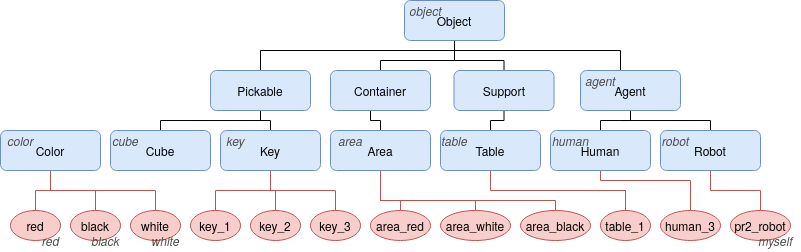
\includegraphics[width=\textwidth]{figures/chapter3/AboxTbox.png}
\caption{The TBox: the types and their hierarchy (in blue), and a part of the ABox ($A$ and $C_0$): the entities and their types (in red), of an example of an ontology representing the situation depicted in Figure~\ref{fig:chap3keys}.}
\label{fig:chap3aboxtbox}
\end{figure}

\begin{figure}[hbtp]
\centering
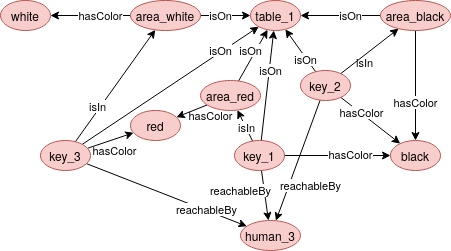
\includegraphics[width=0.8\textwidth]{figures/chapter3/ABoxR.png}
\caption{A part of the ABox ($A$ and $R$) of an example of ontology representing the situation depicted in Figure~\ref{fig:chap3keys}(a).}
\label{fig:chap3aboxrel}
\end{figure}

\paragraph{Ontology definition}
An ontology is a data representation used in many domains. In robotics, it is now widely used as a knowledge base. It is richer than a ``flat'' key-value (or vector) of facts. Indeed, it allows to represent multiple concepts inheriting from one another and entities as the instantiation of these concepts. Moreover, the entities can be linked through properties representing relations. Reasoners can use this structure to deduce other facts through first order logic (\textit{e.g.}~if a key is in an area then the area contains the key; if the key is in an area and the area is on the table then the key is on the table) and add them to the ontology. Recently, ontologies are even standardized for robotic applications such as the IEEE-SA P1872.2 Standard for Autonomous Robotics Ontology.

Formally, as coined by Fokoue \textit{et al.} \cite{fokoue2006summary} and Kr\"otzsch \textit{et al.}, a knowledge base ontology is defined by the tuple $K = \langle \abox, \tbox, \rbox \rangle$. 
The \textit{TBox} $\tbox$ contains the concepts, called \textit{classes} representing the possible types of entities known by the agent. More specifically, it is a finite directed acyclic graph (DAG) $\tbox = \langle T, H \rangle$ with $T$ the set of classes/types and $H$ the directed edges representing the inheritance/inclusion links between them. For simplicity purposes, we will refer to them as ``\textit{isA}'' links. For instance, in an ontology representing the example depicted in Figure~\ref{fig:chap3keys}(a), we have: 
\begin{multline*}
\{Key, Table, Area, Object, Agent, Pickable, Robot, Human\} \subset T,\\
\{(Key, Pickable), (Pickable, Object), (Table, Object),\\
(Robot, Agent), (Human, Agent)\} \subset H
\end{multline*}
(\textit{i.e.}~(\textit{Key}, \textit{isA}, \textit{Pickable}), (\textit{Pickable}, \textit{isA}, \textit{Object}), (\textit{Table}, \textit{isA}, \textit{Object}), (\textit{Robot}, \textit{isA}, \textit{Agent}), (\textit{Human}, \textit{isA}, \textit{Agent})) as represented by the blue graph in Figure~\ref{fig:chap3aboxtbox}.

The RBox $\rbox = \langle P, Incl, Inv \rangle$ contains the properties, their inheritances and inverses known by the agent. $P$ is the set of properties, $Incl$ the finite DAG representing inheritances/inclusions between the properties and $Inv = \{(p_i, p_j) \in P^2\}$ representing the inverse properties. The properties can denote both the attributes of objects (\textit{e.g.}~the color) and the relations between the objects (\textit{e.g.}~which object is on which other one) In an ontology representing the example depicted in Figure~\ref{fig:chap3keys} the RBox may include: 
\begin{multline*}
\{isIn, hasIn, isOn, hasOn, geometricProperty\} \subset P,\\
\{(isIn, geometricProperty), (hasIn, geometricProperty),\\
(isOn, geometricProperty), (hasOn, geometricProperty)\} \subset Incl,\\
\{(isIn, hasIn), (hasIn, isIn), (isOn, hasOn), (hasOn, isOn)\} \subset Inv
\end{multline*}
Note that to fully match the definition of Fokoue \textit{et al.} \cite{fokoue2006summary} it would require to declare the disjunctive, transitive, reflexive and chain relations in $\rbox$ and the disjunctive classes in $\tbox$. As they will be reasoned upon in this thesis, we chose to omit them.

Finally, the ABox $\abox = \langle \indivset, C_0, R \rangle$ contains the entities, their types and relations. $\indivset$ is the set of entities. $C_0 = \{(a, t)|a \in \indivset, t \in T\}$ contains the direct types of each entities (an entity must have at least one direct type, but can have multiple ones). Finally $R = \{(s, p, o)|(s, o) \in \indivset^2, p \in P\}$ is the set of relations between entities. $s$ is called the \textit{subject} of the relation, $p$ the \textit{property} and $o$ the \textit{object}. The relations set $R$ actually contains both attributes of objects (\textit{e.g.}~$(key\_1, hasColor, red)$) and relations between objects (\textit{e.g.}~$(key\_1, isOn, table\_1)$) in our case. For example, in an ontology representing the example of Figure~\ref{fig:chap3keys}(a) we would have as part of the ABox: 
\begin{multline*}
\{key\_1, key\_2, area\_red, table\_1, human\_3, pr2\_robot\} \subset \indivset,\\
\{(key\_1, Key), (key\_2, Key), (area\_red, Area), (table\_1, Table),\\
(human\_3, Human), (pr2\_robot, Robot)\} \subset C_0 \text{ (red part of Figure~\ref{fig:chap3aboxtbox})},\\
(key\_1, isOn, table\_1) \in R \text{ (Figure~\ref{fig:chap3aboxrel})}
\end{multline*}
By using the hierarchy of types we also define $C$ representing the graph of direct and inherited types of entities. $C$ is constructed by adding all the types that can be reached from a direct type of an entity by following a path in $H$. For example $(key\_2, Key) \in C_0 \implies (key\_2, Key) \in C \land (key\_2, Pickable) \in C \land (key\_2, Object) \in C$ if we reuse the example $H$ presented before.
We define the ``isA'' property for simplicity purpose. The ``isA'' property allows to represent hierarchy of types and entities types (as defined in $C$) while only representing triplet, as typical relation (\textit{e.g.}~$(key\_2, isA, Key)$, $(key\_2, isA, Pickable)$, $(key\_2, isA, Object)$. This definition is only intended to help with the notation.
It is important to note that the \textit{id} of an entity must remain internal to the robot and is not intended to be communicated. It is a unique identifier that can be shared across all the robotic architecture. In our examples (and in practice) we use meaningful ids in order for the ontology to be understandable when analyzing it.

In what follows we will consider the TBox and RBox as static. They will be defined before any experiment and will not be modified at runtime. In our architecture, they contain the semantic knowledge of the robot and are not meant to change during a scenario (we do not consider cases where the robot would learn about new categories of objects or about unknown attribute types of objects). The ABox, on the other hand, will contain both predefined entities and relations but also sensed entities and computed facts. It will contain usual symbolic facts, computed by the situation assessment, found in the knowledge bases of typical robotics architecture. However, thanks to their typing and the hierarchy of both types and properties deduction and reasoning can be done on them.

In this thesis we will not present the different reasoners of the ontology, but rather assume that the ontologies used are all been preprocessed and are consistent (\textit{e.g.}~if a relation is in $R$, all the inverse properties of this relation have been added to $R$). More in depth descriptions and uses of ontology in robotic architecture can be found in~\cite{sarthou2019ontologenius} and in Guillaume Sarthou's thesis.

\paragraph{\sparql{} queries}
In addition, ontologies often come with a way of requesting data upon them. A common way of doing so is using \sparql{} queries. \sparql{} queries allow to bind variables with classes or entities respecting the relations specified in the request. The syntax which we will follow in this thesis is for the variable names to begin with a question mark. Let define a \sparql{} query: 
\begin{multline*}
SELECT \ ?key\\
WHERE \{?key \ isA \ Key. \ ?key \ isOn \ table\_1. \ ?key \ hasColor \ black\}
\end{multline*}
This query, issued on the ontology representing the scene depicted in Figure~\ref{fig:chap3keys}(a), would return \textit{\{(key\_1), (key\_2)\}}. Indeed, the first clause\footnote{Actually, \sparql{} engines do not necessary process the clauses in the order they were submitted. Requests are often analyzed and their processing optimized to get the best performance.} \textit{?key isA Key} would lookup for all the entities which are inhering from the \textit{Key} class (Figure~\ref{fig:chap3aboxtbox}). At this stage, \textit{?key} can thus be bound to \textit{key\_1}, \textit{key\_2} and \textit{key\_3}. The second clause, \textit{?key isOn table\_1}, make the \sparql{} engine lookup for entities from the previous set being subject of a relation having as property \textit{isOn} and as object \textit{table\_1} in $R$ (Figure~\ref{fig:chap3aboxrel}). All the entities previously returned does have that relation, so for now \textit{?key} can still be bound to \textit{key\_1}, \textit{key\_2} and \textit{key\_3}. The last clause \textit{?key hasColor black} would again make the engine lookup in $R$ (Figure~\ref{fig:chap3aboxrel}). \textit{key\_3} does not have the relation \textit{hasColor black} so it is removed from the possible bindings of $?key$. The final result is thus \textit{\{(key\_1), (key\_2)\}}. 

A more complete example would be the query:
\begin{multline*}
SELECT \ ?key \ ?area\\
WHERE \ \{?key \ isA \ Key. \ ?area \ isA \ Area. \ ?key\ isIn \ ?area.\}
\end{multline*}
Again, thanks to the first clause ,\textit{?key} can thus be bound to \textit{key\_1}, \textit{key\_2} and \textit{key\_3}. For the second clause, we need to find all the entities inheriting from \textit{Area} in the ABox (Figure~\ref{fig:chap3aboxtbox}). This results in the variable \textit{?area} being possibly bound to \textit{area\_red}, \textit{area\_white} and \textit{area\_black}. For the last clause, possible bindings combinations of both variables are processed, and if $R$ (Figure~\ref{fig:chap3aboxrel}) contains a relation linking them with the \textit{isIn} property, the couple is added to the set of results. The full query thus returns \textit{\{(key\_1, area\_red),(key\_2, area\_black), (key\_3, area\_white)\}}


\paragraph{The multi-agent case}
Finally, we want to be able to estimate and reason on the human beliefs. To do so, we will use one knowledge base (\textit{i.e.}~ontology) per agent considered by the robot in addition to its own. To follow the notation of Chakraborti \cite{chakraborti2018human} presented earlier in this thesis, we will note $K^R = \langle \abox^R, \tbox^R, \rbox^R \rangle$ the knowledge base of the robot and $K^H_r = \langle \abox^H_r, \tbox^H_r, \rbox^H_r \rangle$ the robot estimated knowledge base of the human it is interacting with. In practice, we will have $\tbox^R = \tbox^H_r$ and $\rbox^R = \rbox^H_r$, and only have differences in the ABoxes. Indeed, we assume that the robot estimates that the human knows the same concepts (classes and properties along with their inheritances) as itself. Only the relations between the entities can differ. While this requirement is not needed in our approach, we assume it for clarity purposes.

% Content of the ontology
\paragraph{The content of the ontology in HRI}
The content of the ontology should be carefully chosen for \acrshort{hri}. In our architecture, the content of the robot ontology can be decomposed into three parts (usually not exclusive). 

First, there are the classes and properties used for consistency and to reason on the represented world state. They correspond for example to the inheritance of properties, disjoint classes, inverse properties. 

Then, some classes and properties are dedicated to the ``programming'' of the robot. They allow to abstract some facts in the knowledge base in such a manner that other components can easily access the data they need. For example, the \textit{Container} and \textit{Support} classes can be used by a task planner to easily retrieve objects in the environment that can contain other objects or on which other objects can be placed. Another example can be the \textit{hasMesh} property, allowing the components of the architecture (\textit{e.g.}~motion planner, situation assessment) to share the same geometrical model of an entity.

Finally, some classes and properties are more \acrshort{hri} oriented as they allow to make the interface between the robot knowledge representation and the human. They allow to verbally communicate about entities, to understand situated dialog or to draw the scene for example. They include the classes such as \textit{Cube}, \textit{Key}, \textit{Color} and properties such as the label of entities or \textit{hasColor}.

It is clear that some of the knowledge does not intend to be communicated to the human, however, it can still be in their estimated ontology. For example, the \textit{hasMesh} property cannot be verbally communicated but is in the human estimated ontology as it allows to represent how the human may perceive an object, and allow for perspective taking.


\subsection{REG Features for Communication Action Estimation During Task Planning}
We saw previously that \acrshort{reg} is an important and interesting problem for human-robot interaction scenarios. However, as its application will be on an environment perceived in real-time, along with a collaborative task and with respect to a specific human, additional constraints have to been considered.

\begin{figure}[hbtp]
\centering
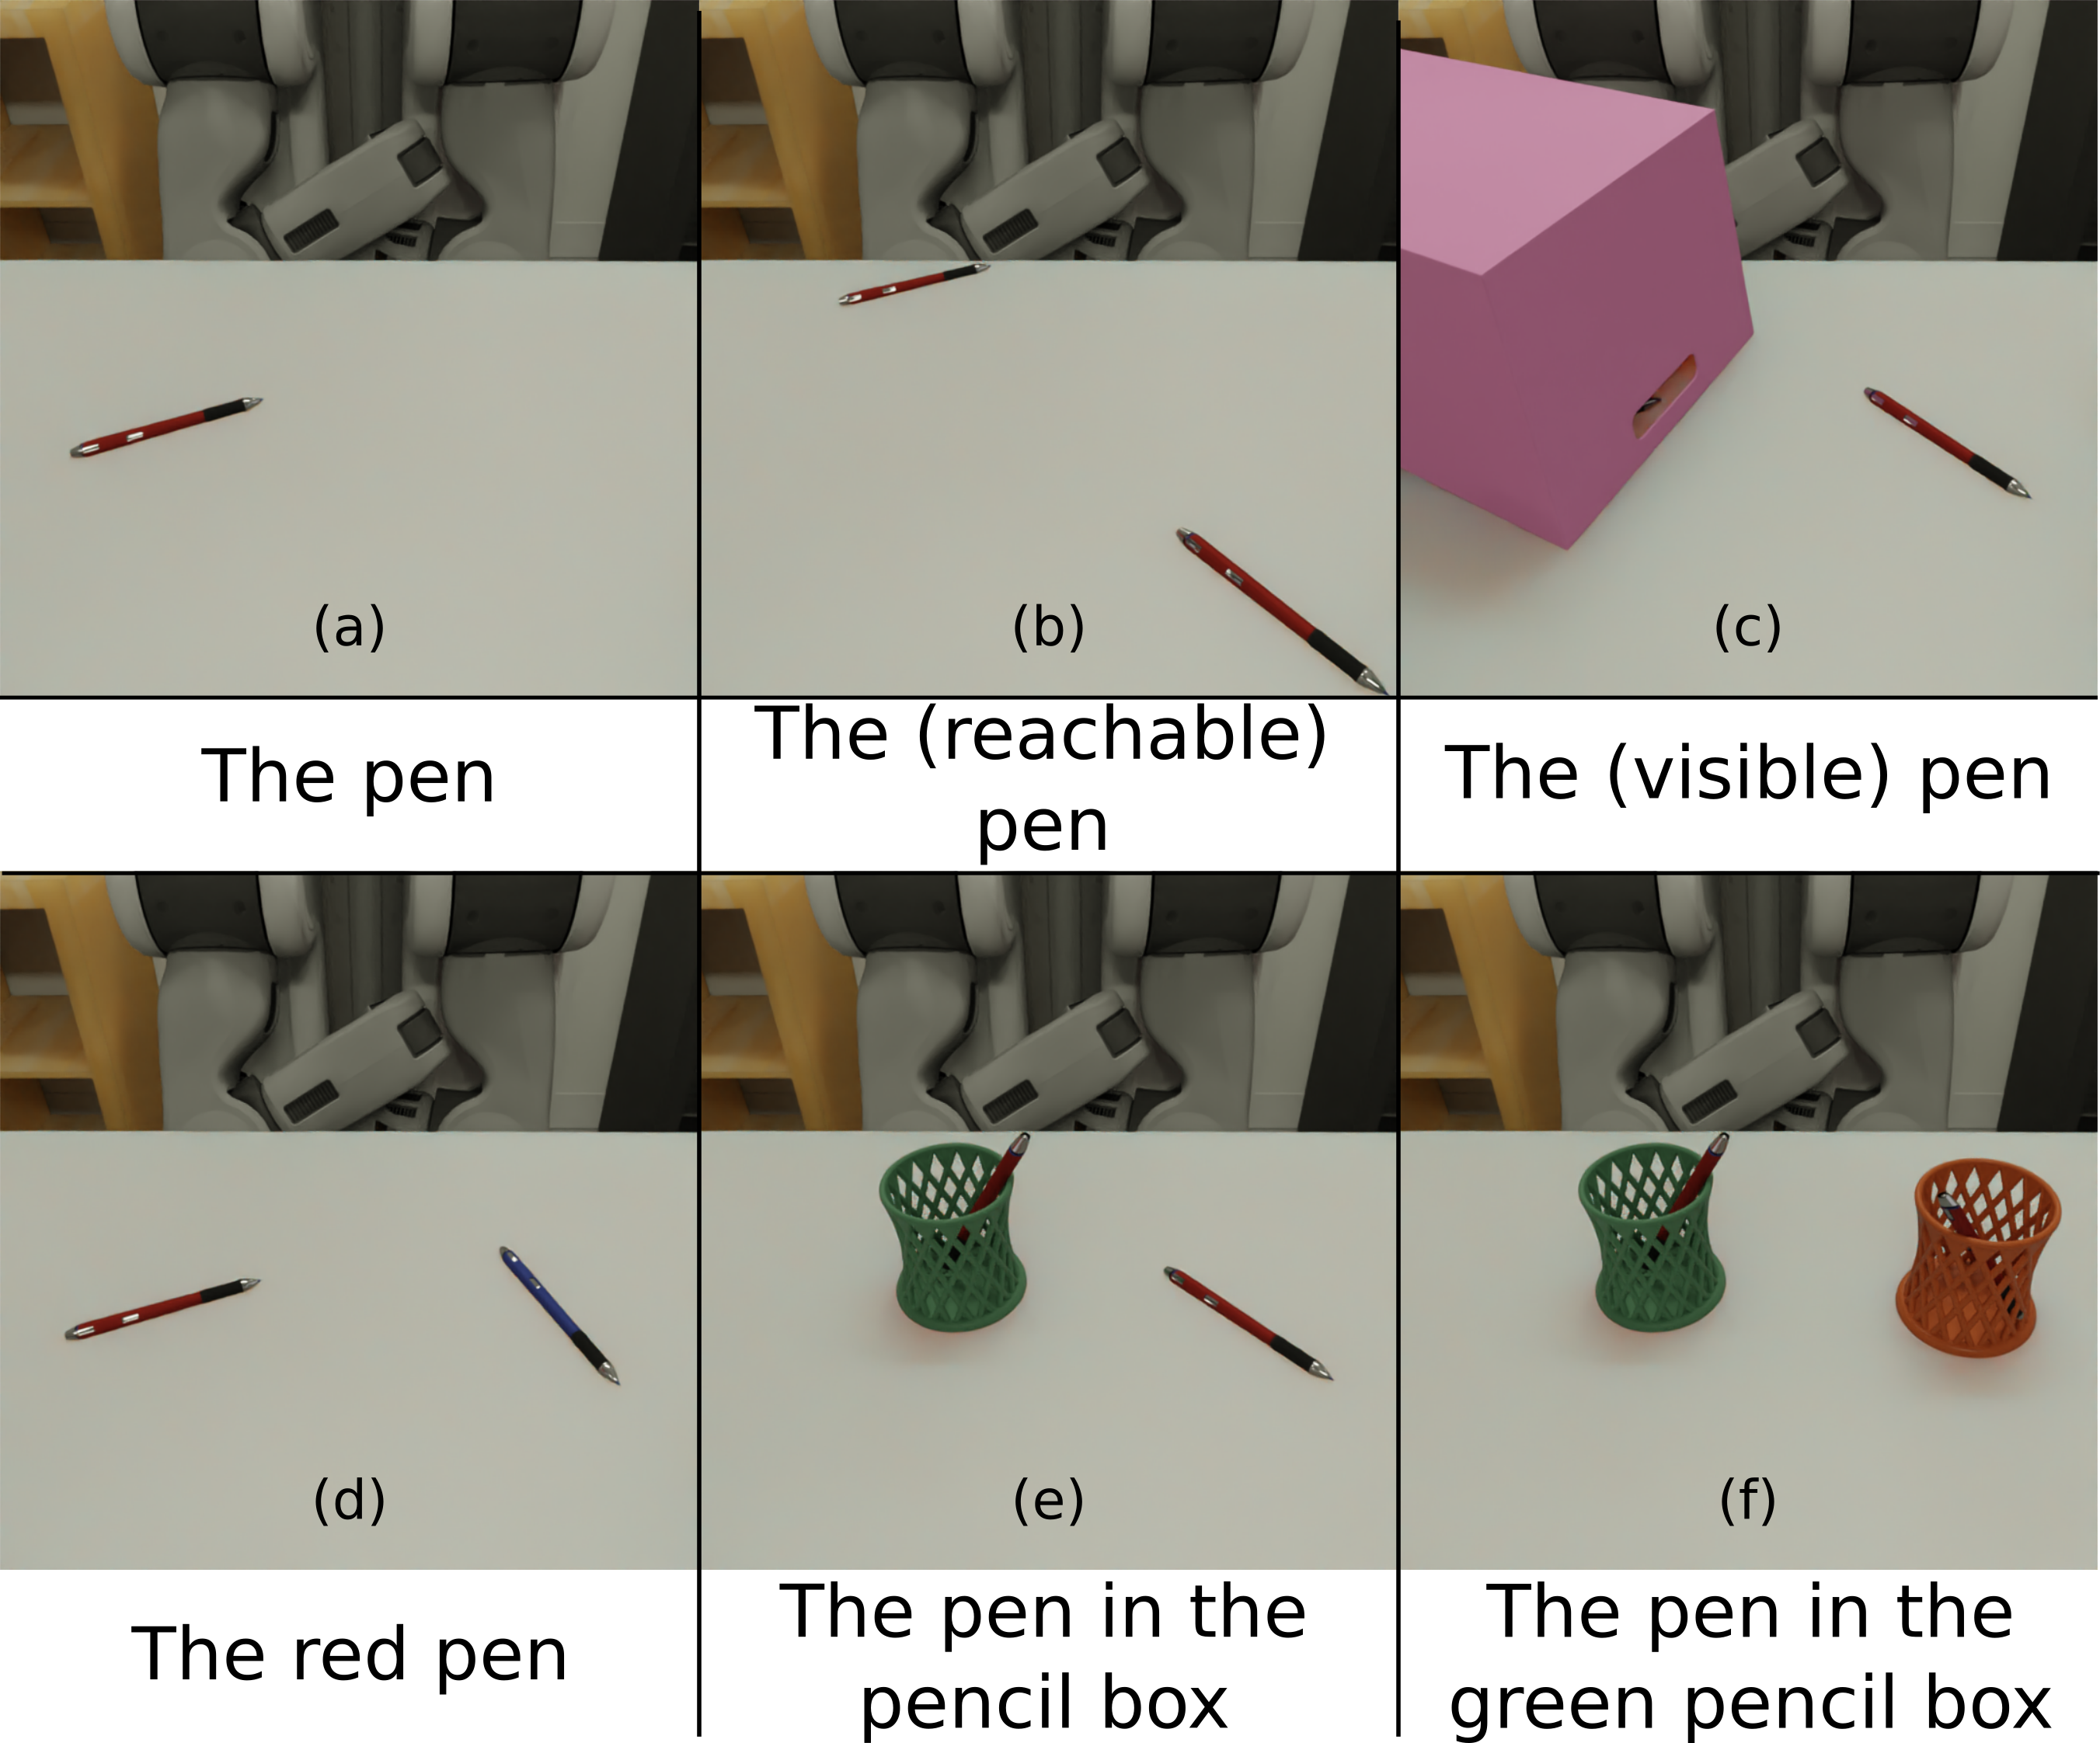
\includegraphics[width=0.7\textwidth]{figures/chapter3/pens.png}
\caption{Six scenes as viewed by a human interacting with a robot at the other side of a table. In each scene, the configuration of objects leads to different mechanisms to refer to a pen without ambiguities.}
\label{fig:pens}
\end{figure}

\begin{enumerate}


\item We want to be able to \textbf{use the relations between entities}. Indeed, we saw that some state of the art approaches were able to only use the attributes of entities in their referring expression and not the relations between them. For instance in Figure~\ref{fig:pens}(e) and (f) the pen can only be referred to by using its relations to the pencil boxes. 
\item Then, we want the algorithm to \textbf{run on existing knowledge bases}. Many presented approaches rely on a dedicated knowledge representation. Such representation can be cumbersome to maintain during an interaction in an evolving environment. Moreover, as stated before, the ontologies used in \acrshort{hri} may already contain the knowledge needed to perform the REG (but often much more). 
\item We also want to support the \textbf{preference ordering} per agent. Indeed, some relations are understood better and quicker than others, and this preference can change depending on the agent we are interacting with. 
\item In addition, we want the algorithm to consider the verbalization through \textbf{the use of types}. All the approaches presented before only focus on the content determination of the \acrshort{reg} and consider that the linguistic realization (the verbalization) will be perfect. They consider that all the contents of the used graph (often dedicated to \acrshort{reg}) can be verbalized (\textit{e.g.}~it exists a word for every edge of the \acrshort{reg} graph and each word correspond to only one edge). While this can be assumed when dealing with a dedicated knowledge base, in an ontology we need the type of an entity as the minimal information needed to refer to an entity (\textit{e.g.}~the \textit{pen\_6} in Figure~\ref{fig:pens} (a) cannot be verbalized directly as ``pen 6'', only its type can be verbalized as ``the pen'').
\item Likewise, in large robotic ontologies, every type or relation cannot be verbalized. Indeed, we saw that they also can contain data to be used by other components (\textit{e.g.}~planners) or to be shared across the architecture. For instance we do not want the robot to say \textit{Pickable} type, the \textit{geometricProperty} or the \textit{hasMesh} property. Thus, our algorithm should be able to \textbf{select only verbalizable types and properties}.
\item Finally, in an interaction, it is clear for the hearer that some entities will not be referred, and should not be taken into account as distractors by the algorithm (in the example depicted in Figure~\ref{fig:pens}(a), it should be clear to the human that, unless specified otherwise, if the robot asks about a pen, it is one on the table and not one in another room). Also, some relations will be implicit in the communication (\textit{e.g.}~if the robot asks the human to \textit{give} it a pen, it is implied that the pen is not reachable by the robot and reachable by the human, as in the Figure~\ref{fig:pens}(b) and (c)). Thus, the algorithm must \textbf{use the context of the ongoing task}. 

Determining the right context (what are the implicit relations, which do not need to be said) is an open challenge. It appears to be linked to the location of the agents and to the action intended to perform with the referred object. We think \textit{affordances} of objects can be a way of determining this context \cite{gibson2014ecological, norman2013design}. Indeed, by emulating the perceived affordances of the different objects perceived by the human, we can deduce which one would be filtered out when asking to perform an action with a referred object. For instance, if the robot asks the human to place the object they are holding on top of a referred object, the human will probably not consider all the object not providing a support as an affordance, the implicit communication would be that the referred object is a support. For now, some affordances are represented as classes in the ontology (\textit{e.g.}~\textit{Pickable}, \textit{Support}). While some effort has still to be put in clearly defining and determining the context for each referring expression, in this thesis the contexts will be deduced by hand and provided to the \acrshort{reg} algorithm.

\end{enumerate}

\subsection{Ontology Based REG Problem Definition}
To formally define the \acrshort{reg} problem for \acrshort{hri}, we need to enhance our knowledge base with three functions.
First, we define a class labeling function $\labelfunc_t: T \mapsto str \cup \bot$ where $str$ denotes a set of character strings used as words in the common human robot vocabulary. We define that a class $t \in T$ is labeled iif $\labelfunc_t(t) \neq \bot$ and call $\labelfunc_t(t) \in str$ the label of $t$. Besides, we require this label to be unique, \textit{i.e.}~for any pair of labeled classes $t, t' \in T^2, t \neq t' \Leftrightarrow \labelfunc_t(t) \neq \labelfunc_t(t')$. We define similarly a an entity labeling function $\labelfunc_a: \indivset \mapsto str \cup \bot$ associating some entities to their speakable/writable unique names (gray names in Figure~\ref{fig:chap3aboxtbox}). These functions can be defined in the ontology by using the commonly used property \textit{rdf:label} to the labeled classes and entities. Adding them that way, allows to make these function agent dependent. In the example depicted in Figure~\ref{fig:chap3keys}(a) we would have among others $\labelfunc_t(Table) = "table"$, $\labelfunc_t(Pickable) = \bot$ and $\labelfunc_t(Key) = "key"$. Indeed, the types and entities are defined by their identifier in the ontology, however these identifiers usually make no sense to the human (\textit{e.g.}~\textit{key\_1}), or are not intended to be verbalized (\textit{e.g.}~\textit{Pickable}). The labels serve to distinguish the individuals and types that are verbalizable from the other and to give a unique verbalizable name to them. In practice, entities are rarely named except for very specific objects that would have been given a unique name.

Moreover, to support the preference ordering we introduce a \textit{comprehension cost function} depending on the agent $\costcompfunc^H: P \mapsto \realset^{+*}$ assigning a positive cost to properties. It allows to represent that some relations are harder to interpret for the hearer than others. We will not present in this thesis how to compute these costs. However, some approaches manage to estimate this cost and the preference order \cite{belke2002tracking, koolen2012learning}. Belke and Meyer evaluated the reaction times to find if two patterns were different, moreover, they analyzed the referring expression generated by participants when presented with two different patterns to refer to one. They found that differences in object colors (absolute difference) appear to make the distinction easier than differences in the size (relative difference). Besides, people tend to over-specify the \acrfull{re} by specifying the color even when it is not needed. This shows that color attributes should be preferred over size when generating a \acrshort{re} \cite{belke2002tracking}. Koolen \textit{et al.} used a learning approach based on human generated RE to assign costs to the relations used by the Incremental Algorithm and Graph-Based Algorithm~\cite{koolen2012learning}. In what follows, all the properties have a unit cost.

We are aiming to unambiguously designate, through its relations to other entities, an entity $\goalindiv \in \indivset$ in a knowledge base $\knowledgebase$. We will call the entity we are trying to refer to the \textit{target entity} $\goalindiv$.
However, the \acrshort{re} is meant to be used in the context of a task. As stated previously, the \acrshort{re} needs to account for certain implicit relations. This is why the problem must be given a \textbf{context} $Ctx = (R_{ctx}, C_{ctx})$, a set of relations and direct types that are implicit in the current situation, which will be used to reference $\goalindiv$, but not included in the generated \acrshort{re}. For the interactions of Figure~\ref{fig:chap3keys}, the context could be defined as:
\begin{multline*}
Ctx = (\{ \langle \goalindiv, isOn, table\_1 \rangle, \langle \goalindiv, isVisibleBy, human\_3 \rangle,\\
\langle \goalindiv, isReachableBy, human\_3 \rangle \}, \emptyset)
\end{multline*}

With this context, we restrict the disambiguation to the entities present on the table $table_1$ and visible and reachable by \textit{human\_3}, the human partner. Indeed, when engaged in a tabletop scenario, objects on the table are prioritized when designating one. Besides, as the robot asks to move the keys, we model that the human infer that the keys referred to are reachable and visible by him.

\medskip
Finally, to be able to run on our ontologies and select only verbalizable properties, we provide the problem with a set of \textbf{usable properties} $\usablepropset \subseteq P$. Because of properties inheritance $Incl$ all the properties inheriting from the ones in $\usablepropset$ are usable in the problem.

We thus define the \acrshort{reg} problem as follows:
\begin{definition}[The referring expression generation problem]
The \acrfull{reg} problem is a tuple $\regproblem = \langle \goalindiv, \knowledgebase, Ctx, \usablepropset \rangle$ with $\goalindiv \in \indivset$ the target entity, $\knowledgebase$ the hearer's estimated knowledge base as an ontology containing the facts the robot estimates the hearer knows, $Ctx$ the context and $\usablepropset \subset P$ the set of usable properties.
\end{definition}
It is important to note that the knowledge base we use is the hearer's one. Indeed, for the referring expression to make sense, we need to ensure that all the types and attributes used are known to the hearer. We see here that such a problem requires the robot to perform perspective taking.

A solution to the \acrshort{reg} problem is a set of relations (the attribute of object, their relations between them and their type) which could be verbalized afterward. We define more precisely what must be a solution to the \acrshort{reg} problem.
Because some entities (actually the vast majority) are \textit{not} labeled (anonymous,) and thus cannot be referred to directly (their id \textit{e.g.}~\textit{key\_1} is only an internal identifier, and does not make any sense for the human), some of the relations might be under-specified. For instance in Figure~\ref{fig:chap3keys}, the sentence ``the black key'' is under-specified in that ``the key'' does not identify a unique entity but any entity with the class \textit{Key}.
In addition, it might be the case that a unique, anonymous, entity participates in more than one relation, \textit{e.g.}~``the black key on the table''. 
To keep track of anonymous entities in under-specified relations, we introduce a variable set $X$, representing the anonymous entities, just as in \sparql{} queries. Again, we choose a syntax where variables will be prefixed with a question mark (\textit{e.g.}~$?y \in X$).
An under-specified relation is thus a triplet $(s, p, o) \in (X \cup \indivset) \times \usablepropset \times (X \cup \indivset)$, \textit{e.g.}~\textit{(?y, hasColor, black)} where $?y \in X$ is a variable and $black \in A$ is a labeled entity in the knowledge base.


When speaking about anonymous entities, one must know its type to serve as a placeholder in sentences (\textit{e.g.}~``the pen'').
Thus, the solution should associate each variable and a type (previously denoted as ``isA'' relations). For simplicity, we chose to represent them also as triplets: $X \times "isA" \times T$ (\textit{e.g.}~\textit{(?y, isA, Cube)}). 

\begin{definition}[Reference]
\label{def:reference}
Thus, a \textbf{reference} $E$ is a set of triplets, each triplet in $E$ being either an under-specified relation in $(X \cup \indivset) \times \usablepropset \times (X \cup \indivset)$ or a type ascription in  $(X \times "isA" \times T)$.
\end{definition}

For example for the ontology depicted in Figure~\ref{fig:chap3aboxtbox} and Figure~\ref{fig:chap3aboxrel}, $\{(area\_white,$ $hasColor,$ $white)\}$, $\{(?0,$ $isOn,$ $table\_1), (?0,$ $isA,$ $Key)\}$ and $\{(key\_2,$ $hasColor,$ $?0), (?1,$ $hasColor,$ $?0), (?0,$ $isA,$ $Color)\}$ are three references. However, a reference may not be verbalizable as is, nor represent a valid situation of the knowledge base. We thus introduce three constraints:

\begin{constraint}[Nameability of entities]
\label{theo:constraint_1}
Each entity $a \in \indivset$ present in any tuple of a reference $E$ (as first or third component) must have a label: $\labelfunc_a(a) \neq \bot$.
\end{constraint}

For instance for Figure~\ref{fig:chap3keys}(a) with the ontology depicted in Figure~\ref{fig:chap3aboxtbox} and Figure~\ref{fig:chap3aboxrel} a reference being: $\{(key\_3, hasColor, red)\}$ violates the Constraint~\ref{theo:constraint_1}. Indeed, even if $red$ does have a label ($\labelfunc_a(red) = "red"$), $key\_3$ does not ($\labelfunc_a(key\_3) = \bot$, the individual $key\_3$ does not have a gray name in Figure~\ref{fig:chap3aboxtbox}).

\begin{constraint}[Nameability of variables]
\label{theo:constraint_2}
For each variable $x \in X$ present in any tuple of a reference $E$ (as first or third component) there must also be a unique tuple in $E$ specifying one of its labeled type ($(x, "isA", t) \in E$ with $t \in T$ and $\labelfunc_t(t) \neq \bot$).
\end{constraint}

Again, in the situation of Figure~\ref{fig:chap3keys}(a) with the ontology in Figure~\ref{fig:chap3aboxtbox} and Figure~\ref{fig:chap3aboxrel}, the references $\{(?0,$ $hasColor,$ $red)\}$ and $\{(?0,$ $hasColor,$ $red), (?0,$ $isA,$ $Pickable)\}$ respect the Constraint~\ref{theo:constraint_1} ($red$ has a label) but violate the Constraint~\ref{theo:constraint_2}. For the first one, $?0$ is a variable but the reference does not contain an \textit{isA} relation linking it to a type. For the second one, it does contain an $isA$ relation linking the variable $?0$ to a type, but $Pickable$ does not have a label ($\labelfunc_t(Pickable) = \bot$; it does not have a gray name in Figure~\ref{fig:chap3aboxtbox}).

\begin{constraint}[Correct instantiation of variables]
\label{theo:constraint_3}
For a reference $E$ there must exist at least one mapping function $f: X \mapsto \indivset$ of the variables in $E$ into entities in $\indivset$ such that the types and relations linking entities in $E$ are still present in $T$ and $R$ once $f$ has been applied.
In practice, $f$ transforms the under-specified relations of $E$ into fully specified ones that must appear in the knowledge base.
\end{constraint}

As an example, in the context of the Figure~\ref{fig:chap3keys}(a) represented by the ontology depicted on Figure~\ref{fig:chap3aboxtbox} and Figure~\ref{fig:chap3aboxrel}, the reference $\{(?0,$ $isA,$ $Key), (?0,$ $hasColor,$ $white)\}$ respects the Constraints~\ref{theo:constraint_1} and \ref{theo:constraint_2}, but does not respect the Constraint~\ref{theo:constraint_3}. Indeed, the variable $?0$ cannot be replaced by an entity having the specified relation in the given ontology (no entity of type \textit{Key} has the relation \textit{hasColor} with the entity $white$).

We can now define a \textbf{valid reference}:

\begin{definition}[Valid reference]
\label{theo:valid_ref}
A reference $E$ is valid with respect to an ontology $\knowledgebase$ if and only if it respects the constraints \ref{theo:constraint_1}, \ref{theo:constraint_2} and \ref{theo:constraint_3}.
\end{definition}

Besides, we define a solution and a complete solution to a REG problem $\regproblem = \langle \goalindiv, \knowledgebase, Ctx, \usablepropset \rangle$:

\begin{definition}[Referring expression]
\label{def:re}
A solution to a \acrshort{reg} problem $\regproblem = \langle \goalindiv, \knowledgebase, Ctx, \usablepropset \rangle$ is called a referring expression and is a tuple $S = \langle E, x_g \rangle$. $E$ is a valid reference and $x_g \in X$ is a variable, such as for each mapping function $f$ respecting the constraint \ref{theo:constraint_3}, $f(x_g) = \goalindiv$.
\end{definition}

\begin{definition}[Complete referring expression]
\label{def:complete_re}
A complete solution to a \acrshort{reg} problem $\regproblem = \langle \goalindiv, \knowledgebase, Ctx, \usablepropset \rangle$ is a solution where the mapping function $f$ respecting the constraint \ref{theo:constraint_3} is unique.
\end{definition}

In the situation of Figure~\ref{fig:chap3keys}(b), a referring expression for the entity $area\_black$ could be $\{(?0, isA, Area), (?1, isA, Key), (?1, hasColor, black), (?1, isIn, ?0)\}$ with $x_g = ?0$. In this situation, $?1$ can be bound to both $key\_1$ or $key\_2$, (two possible mapping functions), but in either case $?0$ can only be bound to $area\_black$. Thus, this referring expression is not complete.

The aim of the hearer is then to instantiate all the variables from their knowledge to find the entity referred to.

Finally, we define an optimal solution (referring expression) $S^* = \langle E^*, x_g \rangle$ as being the a solution minimizing $\sum_{(s, p, o) \in E^*}\costcompfunc(p)$ over the set of all possible solutions for a \acrshort{reg} problem, where $\costcompfunc: P \mapsto \realset^{+*}$ is the properties cost function defined previously. In this thesis, all the properties will have a unit cost, the optimal referring expression will then be the shortest one.


\subsection{Efficient REG Algorithm Presentation}
We aim at building an algorithm to find a solution to the \acrshort{reg} problem. The algorithm must build a set of relations, from the content of a provided ontology, of which all possible substitution of variables would result, for a specific variable $x_g$ to a unique entity of the ontology, the target entity. We choose to inspire from the previous contributions of \acrshort{reg} and to formalize the problem as a graph search. The nodes of this graph are references (as defined in Definition~\ref{def:reference}), and the transitions (edges) are relations from the ontology being added to this reference.

\subsubsection{Formalization as a Graph Search Problem}
\label{sec:SCFormalisation}

Let \textbf{node} $\node = \langle \mathcal{T}_\node, X_\node, A_\node, \mathcal{S}_\node \rangle$. $\mathcal{T} \subseteq \relationset \cup C$ is a set of triplet relations representing some relations in the knowledge base $\knowledgebase$. $X_\node \subseteq X$ is the variable set used in this node, $A_\node \subseteq \indivset$ is the set of anonymous entities of $\mathcal{T}_\node$ and $\mathcal{S}_\node: X_\node \mapsto A_\node$ is the bijective mapping function linking variables to the anonymous entities they represent. We will note $\mathcal{S}^{-1}(T)$ the resulting \textit{reference} (as defined in Definition~\ref{def:reference}) after the application of $\mathcal{S}^{-1}$ on all the entities in each triplet of $T$ which is also in $A_\node$.
The \textbf{initial node} is specified by the user's query through the $context$ of the problem.
The idea is then to explore these nodes until the reference generated from the node $\mathcal{S}^{-1}(T)$ is valid and solution of the \acrshort{reg} problem.
 
To find all substitution functions defined in the Constraint~\ref{theo:constraint_3}, and thus, all the entities which can be bound to the variables in the reference (what the hearer will do to find the entity referred to), we use the \sparql{} queries presented previously. From any node $\node$ we can construct a \sparql{} query from $\mathcal{S}^{-1}(T)$, and submit it on the knowledge base to know how many entities can bound to the variables of the request. In some sense, the \sparql{} queries can be seen as an emulation of the cognitive process the hearer will do when receiving the \acrshort{re}.
A node $\node$ is a \textbf{goal node} if $\goalindiv$ is the only solution to the variable $x_g$ of the \sparql{} query created from the node (Definition~\ref{def:re}), and possibly all the variables in the \sparql{} query have only one assignation (Definition~\ref{def:complete_re}).

A \textbf{transition} $\transition$ in the unambiguous reference generation problem consists in the insertion of a new triplet $(s, p, o)$ to the set $\mathcal{T}_\node$ of a node $\node$ resulting in the creation of a new node $\node'$. The inserted relation in a node $\node$ can be a typing relation ($p \equiv isA$) or a relation which differs between ambiguous entities in $\node$. 
We define two kinds of difference between ambiguous entities.
\begin{definition}[Hard difference]
A \textbf{hard difference} $a_i \harddiff a_j$ exists when two entities have the same property towards a different entity (i.e~$(a_i, p, b_i) \in \relationset \land (a_j, p, b_j) \in \relationset | b_i \neq b_j$).
\end{definition}

\begin{definition}[Soft difference]
A \textbf{soft difference} $a_i \softdiff a_j$ exists when an entity has a property that is not present for any other ambiguous entity (i.e~$(a_i, p, b_i) \in \relationset \land (a_j, p, \cdot) \notin \relationset$).
\end{definition}

For example, in Figure~\ref{fig:chap3keys}(b) we would have for a hard difference: 
\begin{equation*}
(area\_black, hasColor, black) \in area\_black \harddiff area\_red
\end{equation*}
as both $area\_black$ and $area\_red$ have a relation containing the property $hasColor$ but $area\_black$ has this property with the entity $black$ while $area\_red$ has it with the entity $red$. Then, a soft difference would be: 
\begin{equation*}
(key\_1, isIn, area\_black) \in area\_black \softdiff area\_red
\end{equation*}
as the property $isIn$ is present in this relation concerning $area\_black$ but not present in any relation concerning $area\_red$.

As the hard differences respect the \textbf{open-world assumption} but the soft differences do not, we propose to encourage the use of hard differences when possible by adding an extra cost to transitions coming from soft differences.

Finally, the \textbf{cost} of a node is the sum of the costs of each transition leading to this node. If we assume that each transition $\transition_j$ corresponds to the addition of a triplet $(s_j, p_j, o_j)$ to the set $\mathcal{T}_\node$ of a node $\node$ with a cost $\costcompfunc(p_j)$, the cost to $\node$ is $\costcompfunc_\node = \sum_{(s, p, o) \in \mathcal{T}_\node} \costcompfunc(p)$. 

\subsubsection{Algorithm Presentation}
We chose to perform this search and solve the \acrshort{reg} problem to use a uniform cost search algorithm on the graph presented before.
From an initial node built from the context of the query, the algorithm generates new nodes by adding possibly disambiguating relations to the current node. We use a uniform-cost search which is \textbf{optimal} and \textbf{complete} with positive transition costs and a finite number of entities and properties in $\knowledgebase$. Just like Dijkstra's algorithm, it expands the nodes in increasing cost order until a solution is discovered or the search space is exhausted.
%On this basis, we can use a transposition table with the hash of the explored states and thus detect if a state has already been explored or not.
%Informed search and bidirectional search have been both discarded because no admissible heuristic can be defined and because we can not sample a goal state directly. A breath-first search is optimal when all steps costs are equal because it always expands the shallowest unexpanded node. However, the cost of our actions are directly linked to the cost of the relation they contain, and thus, not always equals. 
%In this case, the breadth-first search is not optimal and is therefore not suited to our problem.
%Unlike the breadth-first search, the uniform-cost search (just like Dijkstra algorithm) expands the node with the lowest cost.
%Therefore, we chose to use a uniform cost search algorithm to find the optimal solution.
%States are expanded in increasing cost order until a solution is discovered or the search space is exhausted.
%Pseudocode of the uniform-cost search for the REG problem is given in Algorithm \ref{alg:ucs}.


\begin{algorithm}[htb]
\begin{algorithmic}[1]
\Function {REG}{$\goalindiv$, $\knowledgebase$, $Ctx$, $U$}
\State $node \leftarrow Ctx$
\State $frontier \leftarrow$ a priority queue of nodes ordered by their \textit{cost}, initialized with $node$ having a cost 0 as only element
\State $explored \leftarrow$ an empty set of nodes
\Loop
	\If{\textsc{IsEmpty}($frontier$)} 
		\State \Return failure		
	\EndIf
	\State $node \leftarrow \textsc{Pop}(frontier)$
	\If{\textsc{GoalTest}($node$)} 
		\State \Return $\mathcal{S}^{-1}(\mathcal{T}_{node})$
	\EndIf
	\State $explored \leftarrow explored \cup node$
	\ForEach{$transition$}{\textsc{GetTransitions($node$)}}
		\State $child \leftarrow \textsc{ApplyTransition}(node, transition)$
		\If{$child \notin explored$ and $child \notin frontier$}
			\State \textsc{Insert}($child$, $frontier$)
		\EndIf
	\EndFor
\EndLoop
\EndFunction
\end{algorithmic}
 \caption{Uniform cost search algorithm for referring expression generation.}
 \label{alg:reg}
\end{algorithm}

The graph search algorithm is presented in Algorithm~\ref{alg:reg}. The different transitions (edges) (\textsc{GetTransitions} function) exploring through the nodes can be of two types. Either the reference $\mathcal{S}^{-1}(T)$ of the node contains some variable that are not typed (violating the Constraint~\ref{theo:constraint_2}) and the function returns a typing (\textit{isA}) relation to be added to the set of relations (\textsc{TypingTransitions} function); or it returns the set of soft and hard differences between the anonymous individuals of the node and the other individuals having matched in the \sparql{} query (\textsc{DifferenceTransitions} function) for their substituting variable. By doing so, we ensure that if a node produces a reference that is not valid (violating the Constraint~\ref{theo:constraint_2}), the next transitions are only dedicated to make it valid through typing (\textit{isA}) relations. Moreover, by only adding relations that are in the ontology $\knowledgebase$ we ensure that all the relations of a node are in the ontology, and thus respecting the Constraint~\ref{theo:constraint_3}). Then, the transitions returned are explored and used to create new nodes (\textsc{ApplyTransition} function). A new node is created by copying the relations of its parent and adding the relation of the transition. Moreover, if the transition adds a new anonymous entity, it creates a new variable and adds the binding to the mapping function, ensuring the respect of the Constraint~\ref{theo:constraint_1}). Finally, when a node is explored, its reference is created using its mapping function, then the validity of the reference is checked and if it is valid, a \sparql{} query is constructed and submitted to the ontology to check if the valid reference is solution; if not, the exploration continues.

The different called functions are presented hereafter and the pseudo-codes are given for the most interesting ones:

\textbf{\textsc{ToQuery}:}
Performs a direct translation of a \textit{reference} into a \sparql{} query.

\textbf{\textsc{SparqlResult}:}
The function that takes a \sparql{} query as input and returns a match table $\mathcal{M}: X \mapsto \mathcal{P}(A)$\footnote{This is a simplification of the result returned by a \sparql{} query, as we do not use the relation between the tuples really returned.} in the way that $\mathcal{M}(x)$ is the set of entities matching the variable $x \in X$ in the given query.

\textbf{\textsc{GoalTest}:}
First, this function checks if the reference produced with $\mathcal{S}^{-1}(T)$ is valid. Then, it constructs a \sparql{} query from a node using the \textsc{ToQuery} function. Then, it submit it to the ontology $\knowledgebase$ with the function \textsc{SparqlResult}. Finally, using the resulting match table, it returns $\top$ (true) if the variable denoting the target entity $x_g$ has only one match, being the target entity $\goalindiv$ ($\mathcal{M}(x_g) = \{\goalindiv\}$) and $\bot$ (false) otherwise.

\textbf{\textsc{GetTransitions}:}
(Algorithm~\ref{alg:gettransitions}) At each step, we consider two kinds of possible transitions. The \textsc{TypingTransitions}~function (Algorithm~\ref{alg:typingtrans}) consisting in the addition of an inheritance (\textit{isA}) relation if at least one entity has no label and no inheritance relation in $\mathcal{T}_{\node}$. Otherwise, the \textsc{DifferenceTransitions} concatenates the transitions from the \textbf{hard difference transitions} (Algorithm~\ref{alg:harddifftrans}) and the \textbf{soft differences transitions} (Algorithm~\ref{alg:harddifftrans} with the $\softdiff$ operator at line~\ref{line:harddiff}). These transitions add relations that differ as hard and soft differences between ambiguous entities for each variable in $\mathcal{M}$.

\begin{algorithm}[htpb]
\begin{algorithmic}[1]
\Function {GetTransitions}{$node$}
\State $transitions\leftarrow$ \textsc{TypingTransitions}($node$)
\If{$transitions \neq \emptyset$}
	\State \Return $transitions$
\EndIf
\State $transitions\leftarrow$ \textsc{DifferenceTransitions}($node$)
\State \Return $additions$
\EndFunction
\end{algorithmic}
 \caption{The pseudo-code of the function returning the different transitions (edges) to explore.}
 \label{alg:gettransitions}
\end{algorithm}

\begin{algorithm}[htb]
\begin{algorithmic}[1]
\Function {HardDifferenceTransitions}{$node$}
\State $transitions\leftarrow$ an empty set of transitions
\State $\mathcal{M}\leftarrow$ \textsc{SparqlResult}(\textsc{ToQuery}($\mathcal{S}_{node}^{-1}(\mathcal{T}_{node})$))
\ForEach{$x$}{$X_{node}$}
	\ForEach{$a$}{$\mathcal{M}(x)$}
		\If{$a \neq \mathcal{S}_{node}(x)$}
			\ForEach{$r = (\mathcal{S}_{node}(x), p, o)$}{$\mathcal{S}_{node}(x) \Delta a$} \label{line:harddiff}
				\State $r_{inv} \leftarrow (o, Inv(p), \mathcal{S}_{node}(x))$
				\If{$r \notin \mathcal{T}_{node} \land r_{inv} \notin \mathcal{T}_{node} \land p \in U$}
					\State $transitions \leftarrow transitions \cup \{r\}$
				\EndIf
			\EndFor
		\EndIf
	\EndFor
\EndFor
\State \Return $transitions$
\EndFunction
\end{algorithmic}
 \caption{Hard difference transitions pseudo-code.}
 \label{alg:harddifftrans}
\end{algorithm}

The $\harddiff$ (resp. $\softdiff$) operator returns all the relations that are hard differences (resp. soft) between two entities as defined in \ref{sec:SCFormalisation}. In the difference actions algorithm, an action can be added only once and must not be present in the current state to avoid redundancy. The inverse relation to the one added by the action is also retrieved from the $Inv$ set defined in the knowledge base and checked if not present in the current state and in the current actions set, again to avoid redundancy. 
%In the example of Figure~\ref{fig:search_example} the relation $(P\_1, isIn, G\_2)$ will be redundant if the relation $(G\_2, hasIn, P\_2)$ has been already used in the current state.

\textbf{\textsc{TypingTransitions}:}
The \textsc{TypingTransitions} function (Algorithm~\ref{alg:typingtrans}) stops at the first entity which has no label nor type. This specificity reduces the branching factor while ensuring that each entity has a label or at least a type. Since typing actions are the first tested in the \textsc{GetTransitions} function, all entities not typed during a first execution will be during the next ones. In the implementation, this function has been optimized by observing that once all the entities from the context are typed, the only entities in $\mathcal{T}_{\node}$ which may not be typed are added as the \textit{object} of a \textsc{DifferenceTransitions}. Thus, by storing the object entity of a transition and only checking if it is labeled or has already been typed (and is thus present in $A_{\node}$) we reduce the complexity of the \textsc{TypingTransitions} function.

\begin{algorithm}[htb]
\begin{algorithmic}[1]
\Function {TypingTransitions}{$node$}
\ForEach{$(s, p, o)$}{$T_{node}$}
\If{$ \nexists x \text{~s.t.~} (s, $"isA"$,x) \in \mathcal{T}_{node} \land \labelfunc_a(s) = \bot$}
\State \Return $\{\ (s,\text{"isA"},t)\ |\ t \in \textsc{UsableClasses}(s)\ \} $ and the creation of a new variable 
\EndIf
\EndFor
\State \Return $\emptyset$
\EndFunction
\end{algorithmic}
 \caption{Typing transitions pseudo-code.}
 \label{alg:typingtrans}
\end{algorithm}

\textbf{\textsc{UsableClass}:}
The function \textsc{UsableClasses} returns the most specific \textit{labeled} classes of an entity $\indiv$, \textit{i.e.}~the set of classes $t \in \classset$ such that $(\indiv, t) \in C$, $\class$ is labeled and there are no labeled sub-classes of $t$.

This strategy differs from the one of \cite{dale1995computational} that prefers the least specific types (so-called basic-level classes).
However, in domain-independent knowledge bases such as ours, their scheme could often result in ``Object'' or ``Thing'' which can lead to confusion.
Furthermore, by being conservative in our estimation of the receiver's knowledge base, we can guarantee that the labels of the considered classes are known to the human partner.
Finally, using the most specific classes might reduce the ambiguities, and thus the branching factor early in the search, without impacting completeness.
Note that the restriction to the most specific classes is not necessary but might reduce the branching factor of the algorithm without impacting completeness.

\textbf{\textsc{ApplyTransition}:}
The \textsc{ApplyTransition} function (Algorithm~\ref{alg:transapply}) creates a new node $\node'$ by applying a transition to an existing node $\node$. It always add the triplet of the transition to $\mathcal{T}_{\node'}$ but, in case of a transition coming from the \textsc{TypingTransitions} function, a new variable is created and added to the mapping function $\mathcal{S}_{\node}$ (line~\ref{line:updatesymboltable} of Algorithm~\ref{alg:transapply}). Indeed, if an entity needs to be typed, it means that it is unlabeled and thus need to be represented through a variable in a valid \textit{reference}.

\begin{algorithm}[htb]
\begin{algorithmic}[1]
\Function {ApplyTransition}{$node$, $transition$}
\State $newnode \leftarrow$ a copy of $node$
\State $(s, p, o) \leftarrow transition$
\If{$p \equiv$ "isA"}
	\State $x \leftarrow$ a new variable such that $x \in X \land x \notin X_{newnode}$
	\State $X_{newnode} \leftarrow X_{newnode} \cup x$
	\State $A_{newnode} \leftarrow A_{newnode} \cup s$
	\State Update $\mathcal{S}_{newnode}$ such that $\mathcal{S}_{newnode}(x) = s$ \label{line:updatesymboltable}
\EndIf
\State $\mathcal{T}_{newnode} \leftarrow \mathcal{T}_{newnode} \cup (s, p, o)$
\State \Return $newnode$
\EndFunction
\end{algorithmic}
 \caption{Transition application pseudo-code.}
 \label{alg:transapply}
\end{algorithm}



\subsubsection{Implementation}

The algorithm has been implemented in C++. This choice was motivated by the performance we want our algorithm to have since we aim at using it during task planning. The software must be able to solve several requests per second.

The interface between the algorithm and the ontology (to compute the hard and soft differences and to make the \sparql{} requests) has been done with the Ontologenius API, ultimately using ROS for low level communications. This allows to have the ontology and the REG algorithm to run on different computers. However, it is important to note that a low-level interface has also been used, linking Ontologenius as a dynamic library and running on the same process to avoid communications latency. This approach, while preventing Ontologenius to be used by other software, allows for the best performance. This is the version used to compare the computation times of our approach with the others in what follows.

Besides, the software has been integrated as a ROS node allowing other components, such as the supervision and the task planner presented later in this thesis, to perform \acrshort{reg} requests in a distributed architecture.

%\unsure{hashmap, only storing last individual if not typed, ...}

\subsection{Results}
We present hereafter the solutions given by our algorithm to the illustrative examples. Then we provide results involving a large scale knowledge base describing a full apartment in terms of execution time, solution length and composition. Finally, we provide comparative performance measures with two state-of-the-art methods on their own domains.

\subsubsection{Solutions Analysis}

\begin{figure}[hbtp]
\centering
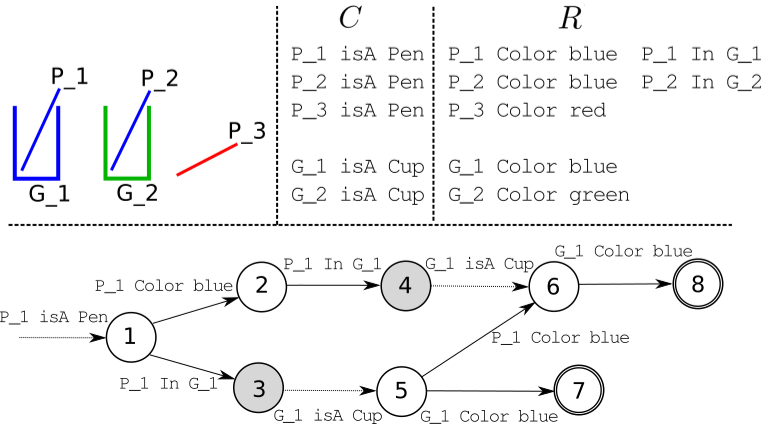
\includegraphics[width=0.7\textwidth]{figures/chapter3/search.png}
\caption{A simple example showing how our ontology-based referring expression generation algorithm explores the search space. The scene is depicted in the top left corner, and \textit{C} and \textit{R} represent respectively the graph of direct and inherited types of the entities and the relations between them. The graph exploration is presented to generate a referring expression for the entity \textit{P\_1}. Dotted arrows represent typing transitions and grayed nodes do not respect \ref{theo:constraint_2}.}
\label{fig:search_example} 
\end{figure}

In order to have a better grasp of the solutions, we propose to present some of them. For every presented solution, the variable denoting the entity to refer to will be $x_g = ?0$.
The first setup is for illustration purpose, and operates on the static knowledge base $\knowledgebase_{pens}$ illustrated in Figure~\ref{fig:search_example}. In this setup, three pens of two colors are represented, two of them are in two different cups of different colors.
Since this setup is really small, the context is always empty, all the relations are usable and no entity is labeled. Moreover, the knowledge base being small, we specify that all the properties $P_{pens}$ are usable.
Thus, based on this setup we propose two \acrshort{reg} problems. The first one $REG_1$ aims at finding a RE for the pen \textit{P\_1}: $REG_1 = \langle P\_1, \knowledgebase_{pens}, \varnothing, P_{pens} \rangle$. The second one $REG_2$ aims at finding a \acrshort{re} for the cup \textit{G\_1}: $REG_2 = \langle G\_1, \knowledgebase_{pens}, \varnothing, P_{pens} \rangle$.
We only tested with two interesting entities since the others present similar characteristics.
The solution for $REG_1$ is \textit{\{(?0, isA, Pen), (?0, isIn, ?1), (?1, isA, Cup), (?1, Color, blue)\}}. For $REG_2$ it is \textit{\{(?0, isA, Cup), (?0, Color, blue)\}}. They can be read respectively as ``the pen in the blue cup'' and ``the blue cup''. These two solutions are complete (as in Definition~\ref{def:complete_re}, allowing to read ``the'' and not ``a'' in the verbalization), as $?0$ and $?1$ bind to only one entity. Here, we see how referring to another entity lead to interesting solutions.

In order to give the reader a sense of how the context is useful as defined in the problem, we propose to come back to Figure~\ref{fig:pens}.
In a knowledge base describing Figure~\ref{fig:pens}(b), with a labeled entity \textit{Bob}, representing the human, giving a empty context to the problem would lead to the solution \textit{\{(?0, isA, Pen), (?0, isReachableBy, Bob)\}}, which would read as ``The pen reachable by Bob''. Whereas, if the robot wants the human to give it the pen, the reachability of the pen is obvious. So the context would become: \textit{\{(pen0, isReachableBy, Bob)\}}, the ensuing solution would be \textit{\{(?0, isA, Pen)\}}, simply verbalizable as ``the pen'', as taking into account the given context resolve the ambiguity.

\subsubsection{Scaling Up}

To assess the relevance of our approach, we created a larger, realistically-sized, knowledge base (101 entities, 36 classes, 40 properties and 497 relations), describing an apartment with three rooms including several furniture (tables, shelves) and objects (cups, boxes) linked through geometrical relations (\textit{atLeftOf}, \textit{onTopOf}) and attributes (color, weight).
%\footnote{The complete ontology is available at [hidden for review]}. 
We ran our algorithm over all the 77 entities inheriting from the ``Object'' class, representing physical entities. 

\newcommand{\us}{$\mu$s\xspace}

As this algorithm must be used in a human robot interaction application, we want it not to spoil the interaction when the robot is computing an explanation. In this setup, 100\% of the entities have been referred in under 4.33ms that is well below 100ms which is the maximum system response time for the user to get a feeling of instantaneity \cite{miller1968response}. Moreover, 50\% are referred under 357\us and 75\% under 772\us (Figure~\ref{fig:scalingup}). On average, 10.6 nodes are explored to refer to an object with an average of 67.35\us/node explored\footnote{Times reported are run on a CPU Intel Core i7-7700 CPU @ 3.60GHz with 32 Go RAM}. These execution times are promising from a combined use with a task planner, as many requests can be performed while planning without slowing too much the task planner.

\begin{figure}[hbtp]
\centering
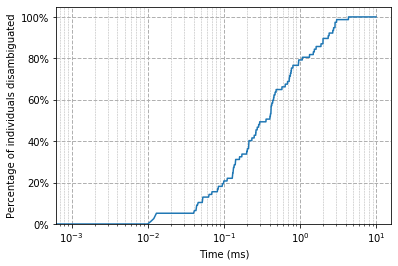
\includegraphics[width=0.6\textwidth]{figures/chapter3/scalingupREG.png}
\caption{Computation times for generating a referring expression on all the 77 objects of the knowledge base representing a three rooms apartment. Orange lines correspond to the minimal size of the RE found at that duration.}
\label{fig:scalingup}
\end{figure}

Over the 77 entities, 32 (41.56\%) are referred to with 2 or less relation meaning that only the type of the entity and one relation is needed to refer to them. We can also note that 25 entities (32.46\%) are referred to using 4 or more relations with a maximum of 6 for one of them. Finally, 49.4\% need to be referred by referring to another entity and two of them need to be referred by referring to two other entities. This means that 49.4\% of the entities can not be referred using approaches like \cite{ros2010one} or \cite{dale1995computational}.

These results over a large scale knowledge base highlight the need to be able to refer to an entity through the use of relation linking it with other entities. They also show that the use of the type of an entity is often sufficient with the use of only one attribute. With this experiment, we also demonstrate that our algorithm is suitable for use with a realistic large scale knowledge base.

\subsubsection{Comparisons With Other State-of-the-Art Algorithms}
\label{subsubsec:REGcomparisons}

\textbf{Longest First} The Longest First (LF)\footnote{http://www.m-mitchell.com/code} algorithm \cite{viethen2013graphs} has been tested on the GRE3D3 Corpus composed of 20 scenes with three objects with different spatial relations relative to one another (\textit{onTopOf}, \textit{atLeftOf}). Each object can be referenced by its color, its size (large or small) and its type (cube or ball). The target referent is marked by an arrow and is always in a direct adjacency relation (\textit{onTopOf} or \textit{inFrontOf}).
Among the 20 scenes, 8 target objects can be referenced without any ambiguity using only their type, 7 can be referenced using only their type in addition to an attribute (color or size) and the other five can be referenced using their types and both color and size attribute. This means that spatial relations are never necessary to reference the target object. 
We perform the comparison on the 19\textsuperscript{th} case which consists of a small green cube on a large green cube and a small blue cube to the right of the green cubes (Figure~\ref{fig:gre3d3}). We chose this case with only cubes because the LF algorithm does not consider the types when generating the RE and adds them only as a post-process. The other cases requiring only the type are resolved in less than 100\us and those requiring the type and an attribute are resolved in less than 250\us with our algorithm.

Since their objective is to obtain an over-specification of the \acrshort{re}, their results are strongly impacted by the maximum length parameter. By setting it to 4 as recommended, we get the result which we can read as ``\textit{The small green cube on top of a cube}'' in 311ms. By setting the maximum length to 3 we obtain the shortest admissible result which can be read as ``\textit{The small green cube}'' in 109ms. This last result is the one given by our algorithm in just 0.87ms.

\begin{figure}[hbtp]
\centering
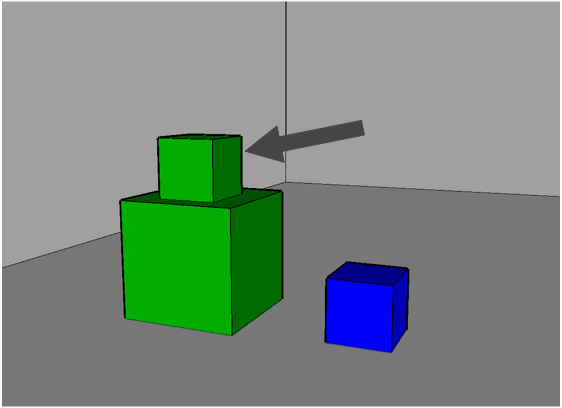
\includegraphics[width=0.4\textwidth]{figures/chapter3/GRE3D319.jpg}
\caption{The scene 19 of the corpus GRE3D3 \cite{viethen2013graphs}.}
\label{fig:gre3d3}
\end{figure}

We see here that the results given by the LF algorithm largely depend on the maximum length parameter. This parameter also has a significant impact on the execution time. Besides, in the realistic scenario presented previously, 13\% of the entity need a reference expression length greater than 4. Thus, even if the over-specification is the goal of the LF approach, it can hardly scale-up. Moreover, for a maximum length fixed at the optimal length, both their approach and ours give identical results.

\textbf{Graph Based Algorithm}
A computationally improved version of the original Graph-Based Algorithm~\cite{viethen2013graphs} is presented in~\cite{li2017automatically}. It aims at extracting, from a dedicated entities relations graph $G$, the lowest cost subgraph which is graph isomorphic to one and only one subgraph in $G$ containing the entity to refer to.
Their approach is evaluated on a corpus containing multiple tabletop scenes \cite{scalise2018natural}, presenting numerous cubes of different colors.

\begin{figure}[hbtp]
\centering
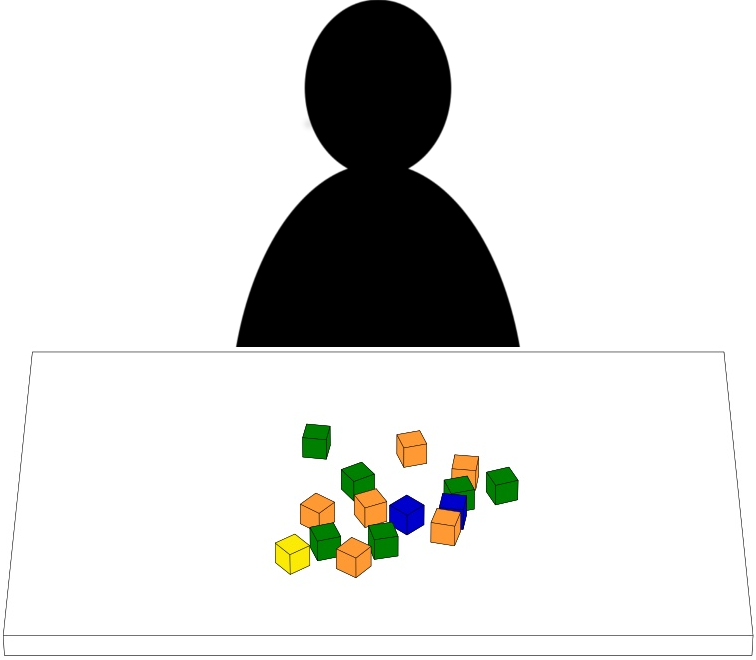
\includegraphics[width=0.5\textwidth]{figures/chapter3/liscene1.png}
\caption{The scene 1 of the Li \& Scalise corpus.}
\label{fig:gbacorpus}
\end{figure}

We generated the graph (relations and costs) used for scene~1 (Figure~\ref{fig:gbacorpus}), converted it into an ontology, and ran our algorithm on it.
This scene contains 15 cubes, GBA algorithm and ours are able to find a solution for the same 10 of them. In all the 10 cases, as we used the same costs, both algorithms returned the same solution (with the types of used entities added in our approach). 
For the other 5 cases, the two algorithms detect the absence of a solution in a few milliseconds.

On all the 10 cases with a solution, our approach performs faster than the GBA algorithm (29.4 times faster on average). We can note that the speed increase is more important in cases where there are many solutions (under 4 times faster on 50\% of the cases, but more than 50 times faster for 25\% of the cases, up to 130 times faster). 
Indeed, the GBA approach uses a branch and bound algorithm where the search graph is bounded if the branch exceeds the cost of the current best found solution. Thus, it can explore a large part of the graph if the optimal solution is not found early in the search. Whereas our approach uses a uniform cost search algorithm, ensuring the first found solution is optimal.
Moreover, we think that in cases where the knowledge base contains entities with different types, our approach should work faster, since we prioritize the use of the type. We were not able to test this, as we could not manage to run the GBA algorithm on other data than their own corpus.

\subsection{Integration}

Our ontology-based \acrshort{reg} method has been integrated on a PR2 robotic platform and used in a tabletop scenario. The used architecture presented in this section is represented in Figure~\ref{fig:regarchi}.

\begin{figure}[hbtp]
\centering
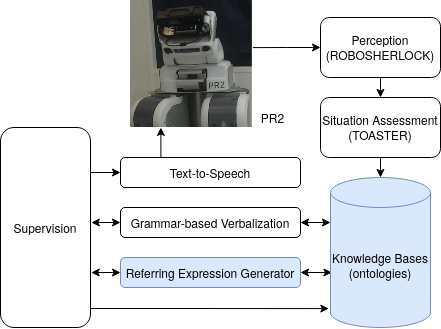
\includegraphics[width=0.7\textwidth]{figures/chapter3/ArchiREG.png}
\caption{The robotic architecture built to test the presented REG approach in real conditions. The blue components are the ones presented in this thesis.}
\label{fig:regarchi}
\end{figure}

The objects on the tables are detected with the ROBOSHERLOCK\footnote{\url{http://robosherlock.org/}} perception system~\cite{beetz2015robosherlock}. This software does not require any a priori on the environment such as CAD model, mesh or training. 
It provides the position (not used to extract relations), the shape (``circular'' or ``rectangular''), represented through a \textit{hasShape} property in the ontology; the color, represented with a \textit{hasColor} property; and the size of the objects (``large'', ``medium'' or ``small''), represented with a \textit{hasSize} property. Since the types of objects is not determined by the system, all the objects were set in the ontology with the labeled type ``Object''. This allows us to challenge our method with situations where the robot is not able to use high-level concepts and where various ambiguities will be raised.

As presented before, the knowledge base is managed using the Ontologenius\footnote{\url{https://sarthou.github.io/ontologenius/}} system \cite{sarthou2019ontologenius}. 
It uses a custom internal structure to store and manipulate assertions as triplets, and offers reasoning capabilities in the form of plugins. Ontologenius provides a low level API allowing to manipulate the knowledge base as a classical data structure in addition to a \sparql{} interface.
The ontology is dynamically fed to keep it up to date on the basis of a simple situation assessment consisting only of filtering and object tracking. The software used is TOASTER, which is an improved version of SPARK \cite{milliez2014framework}. However, only basic capabilities are used, consisting solely of filtering and object tracking. Based on the confidence on the properties extracted, it dynamically feeds the knowledge base to keep it up to date.

A simple linguistic realization has been made, taking as input a \sparql{} query and generating an English sentence as output. For example, it transforms the query ``?0 isA Cup, ?0 isOn ?1, ?1 isA Table, ?1 hasColor black'' into ``\textit{the cup on the black table}''. It is an ad-hoc implementation based on a simple grammar and on the labels contained in the ontology. 

Finally, a supervision component was built by another PhD. student Amandine Mayima. This supervision component orchestrates all the other ones. It receives as input an object being clicked on the RViz visualization, finds its identifier from the ontology, requests the REG component for a referring expression to this object, then sends it to the verbalization component and finally sends the produced sentence to the text-to-speech component making the robot play it.

\begin{figure}[hbtp]
\centering
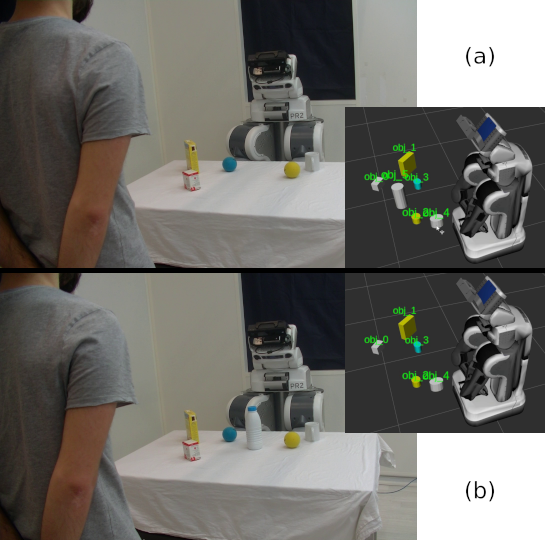
\includegraphics[width=0.8\textwidth]{figures/chapter3/REGIntegration.png}
\caption{The experimental setup for the integration of the \acrshort{reg} algorithm. The robot only perceives the size, color and shape of the objects on the table. It estimates that the human is also aware of these attributes. To refer to the white mug (\textit{obj\_4}) the sentence generated in condition (a) is \textit{``The white circular object''}, while in condition (b) it is \textit{``The white small circular object''}. Indeed, in (a) only the color and the shape of the mug are enough to discriminate it, but in (b) a milk bottle is added, as it is also small and white, the algorithm adds the size of the mug to referring expression.}
\label{fig:setupintegrationreg}
\end{figure}

The task involves six objects on a table (Figure~\ref{fig:setupintegrationreg}). A commented video is available at \url{https://youtu.be/mKDLvDbHfvk}. The entity to reference is \textit{obj\_4} (a white mug). The robot generates the solution ``\textit{The white circular object}'' since there are other non-white circular objects and other white non-circular objects (Figure~\ref{fig:setupintegrationreg}(a)). Then, a human adds a new object which is a white and circular milk bottle (\textit{obj\_5}) (Figure~\ref{fig:setupintegrationreg}(b)). When the robot is asked to describe the white cup, it generates the sentence ``\textit{The white small circular object}''. With this simple task, we show that our REG algorithm can be used within a robotic architecture, can deal with a dynamic environment and can adapt its explanation to the current situation.


\section[Using REG in Task Planning]{Planning Communication Actions Using Referring Expression Generation}

We are now able to determine efficiently the content needed for the robot to refer to an object to a human based on an ontology as knowledge base. Moreover, this algorithm is able to determine if such a communication is feasible (whether it fails or not to find a solution) and gives an estimation of the cost of interpreting the referring expression. In what follows we integrate this approach in a task planner, allowing to evaluate the feasibility and the cost of verbal referring communication actions during task planning.

\subsection{Method}
\label{sec:Integration}

In this section, we first provide an overview of our approach and briefly describe the used Hierarchical Agent-based Task Planner~\cite{lallement2014hatp}. Then, we present the integration of the REG in it and how it allows the planner to be informed of the feasibility and the cost of the communication actions.

\subsection{Approach}


The communication actions that we consider in this paper are instructions issued by the robot to its human partner based on \acrfullpl{re}. Typical instructions are ``\textit{Take X}'' and ``\textit{Put it in Y}''. We thus have a static part and the rest depends on the situation when the communication is performed and must be solved by a REG. It is this variable part that could make a communication costly or infeasible. As stated before, REG must be performed on the human's partner \acrfull{kb} to only use facts and concepts that the robot estimates to be known by the human. Thus, we target a planner that is already suitable for \acrshort{hri} to integrate the estimation of communications. This means that we need a planner able to distinguish between the different agents involved in the task and to maintain a representation of the environment for each of them.

Because the task the planner has to solve does not necessarily imply all the elements present in the current environment, the planner does not need a full representation of the environment. In the same way, it does not necessarily need to have all the characteristics of the entities such that their colors or their types. In the example of Figure~\ref{fig:chap3keys}, the two keys to move can only be represented as movable objects in the planner and not as keys to make the planning domain more generic. 

However, the \acrshort{reg} needs all the semantic information of each entity of the environment to generate accurate \acrshort{re}. Furthermore, if another key which is not part of the task, thus not part of the planner internal representation, is present on the table (such as \textit{key\_3}), it will also impact the \acrshort{reg} and thus the complexity and feasibility of the communication action. 
Hence, the \acrshort{reg} can not be performed on the planner internal representation of the world only.
To solve this issue, we endow the planner with the ability to update a semantic \acrshort{kb} that is used by the \acrshort{reg}. Since maintaining this external representation can be a heavy process, it is updated only when a communication action has to be evaluated.

The general workflow executed for each communication action encountered during the planning process consists of: 1) updating the external semantic \acrshort{kb} of the human partner with the expected world state 2) identifying the objects to which to refer to in the communication 3) execute the \acrshort{reg} for each of these objects 4) calculate the feasibility and the cost of the communication action according to the feasibility and the cost of each individual \acrshort{re} involved in the planned communication. Note that the examples used in this paper only involve one \acrshort{re} but the same method can be used for communications of type ``\textit{give me X and Y}''. In this case, the external semantic \acrshort{kb} is only updated once and both \acrshort{reg} are executed on this \acrshort{kb}.

\begin{comment}

\begin{figure}[hbtp]
\centering
\includegraphics[scale=0.5]{images/workflow.jpg}
\caption{\label{fig:workflow} Workflow to compute the feasibility and cost of a referring communication for each evaluated action involving verbal communication during the planning process.}
\end{figure}

\end{comment}

\subsubsection{Hierarchical Task Planner}

In order to implement our approach, we need a task planner able to maintain an estimated knowledge base of each agent at each planning step. We chose the \acrfull{hatp}~\cite{lallement2014hatp}. \acrshort{hatp} extends the classical \acrfull{htn} planning by being able to produce \textit{shared plans} to reach a joint goal. A \acrshort{hatp} planning domain describes how to decompose tasks into subtasks down to atomic symbolic actions. Both the robot and human feasible tasks and actions are described in the domain. A context-dependent cost function is associated with each action. 

During the task decomposition, \acrshort{hatp} will explore several applicable sub-tasks until the global task is totally refined into feasible actions, and will return the minimal cost plan. \acrshort{hatp} also supports \textit{social rules}, allowing to balance the effort of involved agents depending on human preferences and to penalize plans presenting certain undesirable sequences of actions. We will not use these social rules in what follows, but our approach stays totally compatible with them.

% Task assignation and streams
Moreover, during the exploration of the task tree, \acrshort{hatp} will assign actions to available agents, robot or human (when an action can be done by both). By doing so, \acrshort{hatp} is able to elaborate one action \textit{stream} per agent, together with causality and synchronization links. 
% Multi state variables
Besides, \acrshort{hatp} domain syntax supports Multiple Values State Variables (MVSV)~\cite{guitton2012belief} which is used to represent and reason about each agent mental state. The value of each variable depends on the agent it is requested for. This allows to represent action preconditions depending on the knowledge of the agent performing the action and also to represent their effect on each agent mental state which can depend on the agent perspective.
% GTP

Finally, the last argument which motivated our choice was the previous integration of \acrshort{hatp}  with a  Geometrical Task Planning (GTP)~\cite{gharbi2015combining}. This work aimed at refining geometric and motion planning requests during the task planning process. The geometric planner would then compute, in context, the feasibility, the cost and the side effects of the action. In a similar way, we propose here to integrate and run REG, in context, to determine communication action feasibility and pertinence with respect to other courses of actions.

%Finally, the last argument which motivated our choice was the use of HATP in a previous work: the Geometrical Task Planning (GTP) \cite{gharbi2015combining}. This work aimed at refining into motion planning requests the symbolic motion actions explored by HATP during the task planning process. The motion planner would then returns the feasibility and the cost of the action, but was also able to inform HATP about why the motion action would not be possible (e.g. the object with which collision would occur). The task planner would then, backtrack to choose a different action to remove the colliding object. This method also shows how to update the geometrical planned environment to math the symbolic one in order to run the motion planning phase.
%This also needs to update the geometrical planned world to match the symbolic planned knowledge base before running the motion planning phase. 
%This last work greatly inspired us, and our approach is similar with the difference that we run a REG when a communication action is explored, instead of a motion planning request on a symbolic motion task exploration.

\paragraph{The HATP Data Structures}
As presented in \cite{de2015hatp}, the \acrshort{hatp} data structures are organized around the so-called \textit{HATP entities}. These entities are a collection of any number of attributes being manipulated during the planning process. The \textit{type of the attributes} can either be a basic type (\textit{i.e.}~integer, floating point number, boolean or string) or another entity type. Besides, an attribute can either be \textit{a set}, holding multiple values of the specified type or \textit{an atom}, being a unique element of the specified type. Finally, an attribute can either be set as \textit{static} or \textit{dynamic}. Static attributes cannot be modified once they have been set in the world state initialization, they will only be read during the planning process, whereas dynamic attributes can also be changed by the effects of the primitive tasks (actions). The Listing~\ref{lst:hatpcubes} gives an example of entity definitions in order to represent the situation in Figure~\ref{fig:chap3keys}.

\begin{lstlisting}[caption={Example of a part of the HATP domain describing the situation of Figure~\ref{fig:chap3keys}.}, label={lst:hatpcubes}, emph={define, entityType, entityAttributes, dynamic, atom, set, static}, emphstyle={\bfseries}, captionpos=b, frame=single]
// Agent entity type is implicit
define entityType Cube, Area;
define entityAttributes Cube{
  dynamic atom Area isIn;
  dynamic atom Agent isHeldBy;
}
define entityAttributes Area{
  dynamic set Cube hasIn;
}
define entityAttributes Agent{
  static atom string type;
  dynamic atom Cube isHolding;
}
\end{lstlisting}


\subsubsection{Integration of REG Within Action Planning}
\textbf{The representation of the communication actions:}
% Scénars 
For clarity purposes, we only place ourselves in scenarios where only the robot knows the goal of a joint task and issues command to its human partner one at a time when the human has to do an action. Thus, while planning, if a task is allocated to the human, as she has no way of guessing it, a preceding communication is required. In the \acrshort{hatp} domain, this translates as a method being decomposed into a sequence of a communication action (the instruction to the human) and an action made by the human when the task is attributed to the human. The communication action feasibility is determined by both symbolic preconditions (\textit{e.g.}~the human and the robot are in the same room) and \acrshort{reg} result (whether a solution is found or not). If the communication action is feasible, the cost of the communication action is then computed as the sum of a fixed cost depending on the type of communication and the \acrshort{reg} solution cost depending on the human receiver and the entities to refer to in the communication.

We have chosen here for illustration purposes a simple planning problem where a communication needing a REG is involved in each plan step concerning the human, but the method is general and compatible with problems which need to estimate and ensure the pertinent context and plan step (the \textit{when}) of a communication action during plan elaboration (\textit{e.g.}~\cite{devin2016implemented}, \cite{unhelkar2020decision}).

\textbf{Updating the right knowledge base, at the right time:}
% Ontology et planning KB
On one hand, we have large, complete semantic knowledge bases on which a \acrshort{reg} algorithm is able to run and to return the feasibility, the cost and the content of a verbal entity referring communication for a specified agent (top part of Figure~\ref{fig:integration}). On the other hand, we have reduced knowledge bases dedicated to task planning (bottom part of Figure~\ref{fig:integration}). In order to know the feasibility and cost of a verbal communication action during the planning, we have to reconcile both sides. Indeed, the estimated ontology of the communication receiver must be updated to reflect her planned estimated beliefs at the time of the communication. All the knowledge representation used here are from the robot point-of-view and managed internally by the robot decisional and knowledge management processes.

% Initilization, ne modifions pas l'originale, donc copie de planning
First, the attributes of all the entities present in the planning knowledge base are initialized for each agent (left part of Figure~\ref{fig:integration}). To do so, the name of every \acrshort{hatp} entity types declared in the planning domain are listed. Then, for each entity type, the entities in the ontology inheriting from these types are created in the planning knowledge base. Then, each attribute (both static and dynamic) declared in the domain of every entity has its value updated. If the attribute is a \textit{set}, multiple relations with the same name originating from the same entity and pointing to different ones can be found in the ontology. If so, all the pointed entities are added to the set. If the attribute is an \textit{atom}, only one value is retrieved from the ontology and is set to the planner entity attribute. For instance, if we initialize the planning knowledge base defined in Listing~\ref{lst:hatpcubes} with the content of the ontology depicted in Figure~\ref{fig:chap3aboxtbox} and Figure~\ref{fig:chap3aboxrel} representing the situation of Figure~\ref{fig:chap3keys}, the entity types retrieved from the domain would be \textit{Agent}, \textit{Key}, \textit{Area}, the planning knowledge base would then be initialized with the entities \textit{human\_3}, \textit{pr2\_robot} as Agent; \textit{key\_1}, \textit{key\_2}, \textit{key\_3} as Key; and \textit{area\_red}, \textit{area\_white}, \textit{area\_black} as Area. Then, the attributes of \textit{key\_1} would be retrieved from the ontology and set as $isIn = area\_red$, the same process is repeated for all the other attributes. Attributes that are not in the ontology can be set in the planning domain manually.
Finally, an ontology dedicated to the task planning process (called planning ontology) is created by copy of the present one for every agent other than the robot present in the planning domain. These copies are made to avoid modifying the original ontologies during the planning process as other components may rely on them.


% Pendant la planif ontseules les planning KB sont updates, mais le REG tourne sur l'ontologie complète
%During the task tree exploration (right part of Figure~\ref{fig:integration}), when a communication action needing to refer to entities is encountered, the ontology of the communication receiver needs to be updated for the REG to run on and check whether the referring is feasible and what is its cost.
When a communication action is encountered during the task tree exploration (right part of Figure~\ref{fig:integration}), the ontology of the communication receiver needs to be updated to be able to run the \acrshort{reg} on it.
The planning ontology copy of the receiver human is retrieved by her identifier. Then, for each of the entities of her planned beliefs at the time of the communication, an update is made. The update is only made on \textit{dynamic} attributes as \textit{static} ones do not change during the planning process. All the relations having the same name as the attribute of the entity in the planning domain are deleted from the ontology, and replaced with new planned values. If the attribute is a \textit{set}, a new relation with the same name is created for every value in the set.

A \acrshort{reg} request is then issued on the updated ontology with the goal individual being the entity to refer. The \acrshort{reg} returns a solution with a cost or a failure which is taken into account by the planner as classical cost or a non fulfillment of the action preconditions respectively. Alternatively, a communication action may need to refer to multiple entities. In that case, multiple \acrshort{reg} requests are issued on the same updated ontology and their costs are summed.

With this approach, we are able to change the \textit{context} and \textit{usable relations} provided to the \acrshort{reg} algorithm depending on the task and world state the planner is in. For example, if the human and the robot are in front of the same table, the context would be to consider only entities on that table. Moreover, if the currently explored action is to ask the human for pick, the context provided would be to consider only the \textit{Pickable} objects that are estimated in the human beliefs to be \textit{reachableBy} themselves.

By doing so, we are linking two knowledge bases: the \acrshort{hatp} on one side and the ontology on the other. While the former can hardly represent inheritances between entity types and deduce facts as we do not want to put more load on the task planner, using the latter at specific chosen steps of the task planning process allows to use its rich semantic to make the resulting plan more precise.

\begin{figure}[t!]
\centering
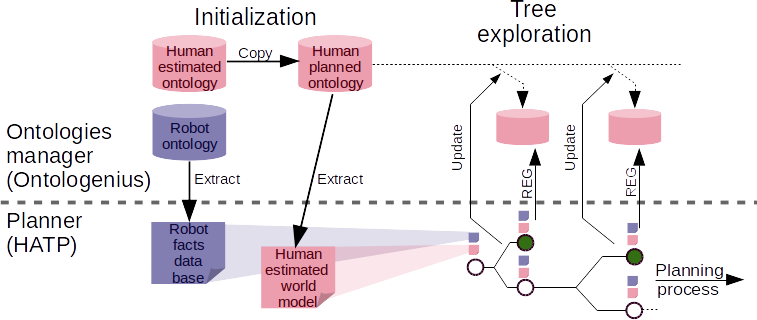
\includegraphics[width=\textwidth]{figures/chapter3/struct.png}
\caption{\label{fig:integration} A representation of the exploration of potential mental states and ontologies conducted by the planner. The ontology representing estimated human knowledge is first copied in order to plan it without altering the original one. The human and robot planning information is extracted from the ontologies. During the tree exploration, for each verbal communication action, the planned human ontology is updated with the current explored state and the REG is executed on it.}
\end{figure}

\subsection{Case Studies}
\label{sec:Case_studies}

In this section, we present three case studies. The two first ones are run in simulation on a minimalist setup and show respectively that the estimation of the communication content during the planning can prevent execution dead-end and can reduce the global communication complexity during the task. The third case study is run on a PR2 robot with a perception of its environment and presents a more complex task with twelve objects to organize. With this last case, we show that our method makes it possible to compare different means of communication and to choose the most appropriate.

To realize tests in laboratory conditions, we chose to replace the keys of Figure~\ref{fig:chap3keys} with cubes (Figure~\ref{fig:chap3scen1}). Thus, all three case studies are based on a cube arrangement task. The human can distinguish the cubes by their color and the digit written on them (one or two) if there is one. As in Figure~\ref{fig:chap3keys}, the table surface is composed of three storage areas of different colors and cubes can be placed only in one of them. This symbolic position information can also be used by the human to distinguish the cubes. In this way, the robot can refer to a cube with a REG of the type: ``\textit{the black cube with the number 2 which is in the black area}''. In all the cases, only the robot knows the goal position of the cubes but can not manipulate them. It thus has to guide the human in the arrangement task. The robot can only point at the cubes in the third case study. In the first two, it can only use verbal communication.

\subsubsection{Preventing Execution Deadlocks}
\begin{figure}[t!]
\centering
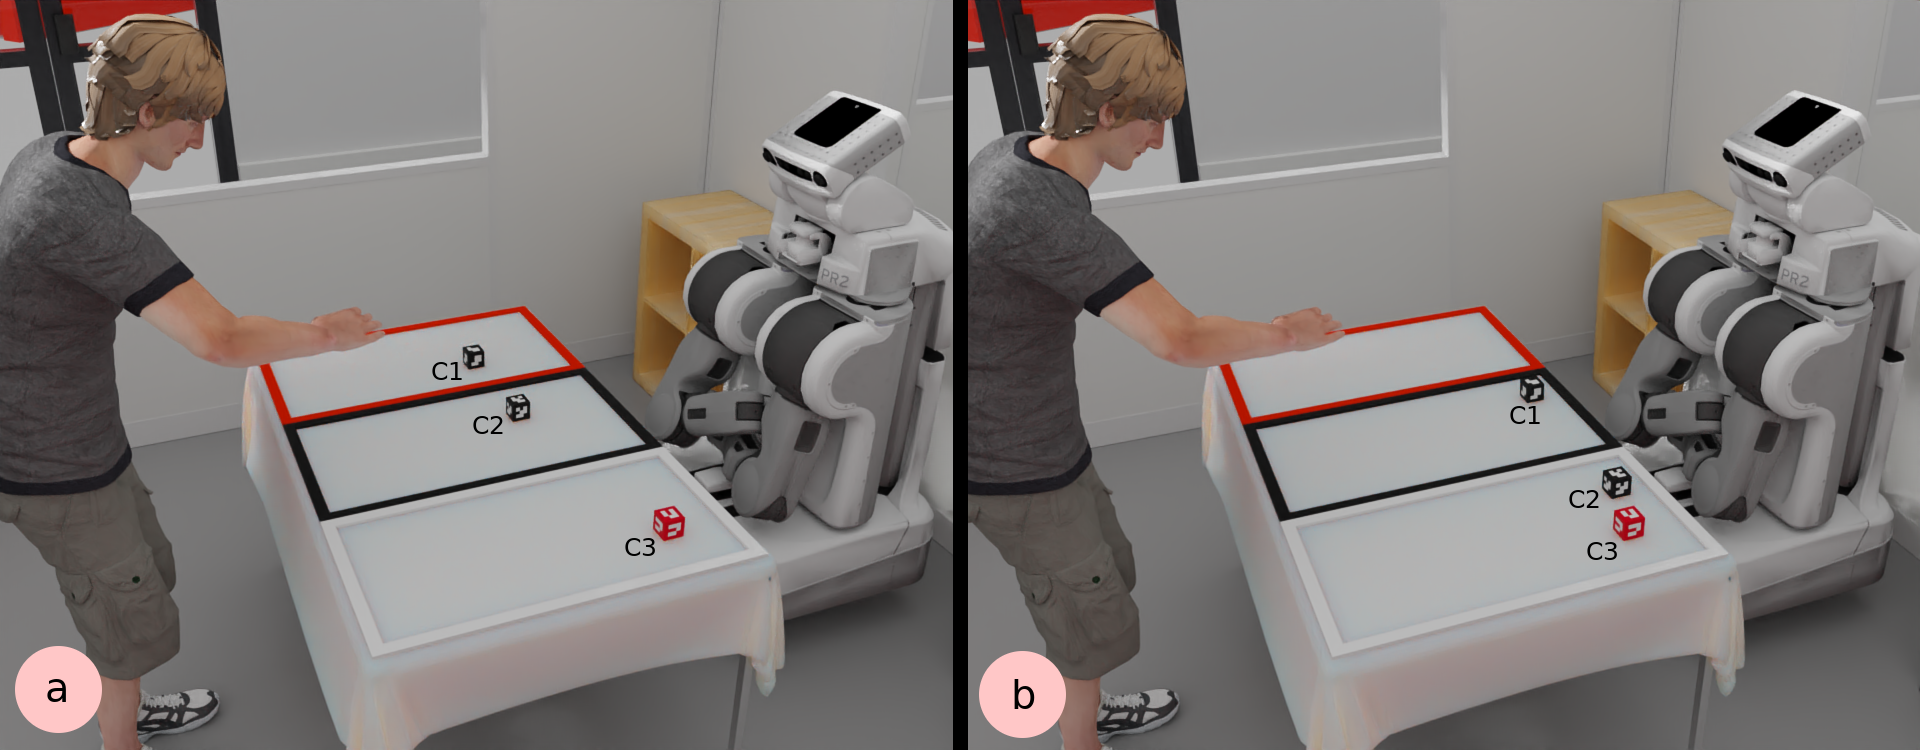
\includegraphics[width=\textwidth]{figures/chapter3/Chap3scen1.png}
\caption{\label{fig:chap3scen1}The situation depicted in Figure~\ref{fig:chap3keys} with keys replaced with cubes to realize the setup in laboratory conditions. The human and the robot are in the situation depicted in (a). Only the robot knows the goal configuration (b) but cannot move the cube. It has to elaborate a plan in which it asks the human to move the cubes.}
\end{figure}
In this case study, we consider the initial state presented in Figure~\ref{fig:chap3scen1}(a). The cube \textit{C1} is in the red area and the cube \textit{C2} in the black one. The goal state is to have the cube \textit{C1} in the black area and the cube \textit{C2} in the white one (Figure~\ref{fig:chap3scen1}(b)).
Taking into account the cost and the feasibility of the communication, the planner elaborated the plan presented in Listing~\ref{list:case1}. Cube \textit{C2} is moved first because otherwise the two cubes would be in the black area at the same time. Such a situation would cause a dead-end during the execution of the plan or require another communication mean.

%footnotesize
\begin{lstlisting}[frame=single, basicstyle=\scriptsize\ttfamily, caption={The obtained plan for the first case study where cube C1 must be moved from the red to the black area and cube C2 moved from the black to the white area. The lines beginning with H represent the actions of the human and the lines beginning with HR represent actions involving the human and the robot (communication actions). In green are the REG results for each communication action.},captionpos=b, style=customPlan, label={list:case1}]
HR - TellHumanToTake(C2) // (?0, isA, Cube), (?0, isIn, ?1), 
                         // (?1, isA, Area), (?1, hasColor, black)
H  - Take(C2)
HR - TellHumanToPlace(C2, AW) // (?0, isA, Area),  (?0, hasColor, white)
H  - Place(C2, AW)
HR - TellHumanToTake(C1) // (?0, isA, Cube), (?0, isIn, ?1), 
                         // (?1, isA, Area), (?1, hasColor, red)
H  - Take(C1)
HR - TellHumanToPlace(C1, AB)  // (?0, isA, Area), (?0, hasColor, black)
H  - Place(C1, AB)
\end{lstlisting}

We consider once again the initial state presented in Figure~\ref{fig:chap3scen1}(a). This time the goal is to invert the positions of the two cubes. In this situation, if the communication cost and feasibility are not taken into account during planning, both actions directly leading to the goal state (\textit{i.e.}~cube \textit{C1} moved to the black area or cube \textit{C2} to the red area) will lead to a deadlock at plan execution. Indeed, regardless of the first cube moved, if it is moved directly to its goal position, it will end up in the same area as another cube of the same color. In such a situation, no \acrshort{re} can be found for the other cube, leading to a deadlock in the execution.
The solution found with our method is to add a supplementary action. It consists of putting the cube \textit{C1} away (in the white area). This additional action avoids a deadlock by making the referring to the cube \textit{C2} feasible.

\subsubsection{Reduction of the Overall Communication Complexity}

\begin{figure}[t!]
\centering
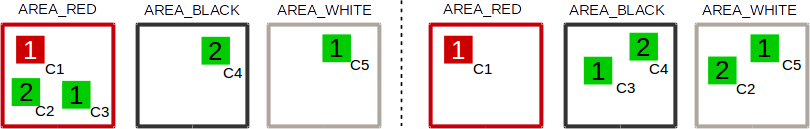
\includegraphics[width=\textwidth]{figures/chapter3/setup2.png}
\caption{\label{fig:case2} The initial state (left) and the goal state (right) of a task where the robot has to explain to the human partner how to move the cubes to complete the task. }
\end{figure}

In this second case study, we show how the estimation of communication by verbal designation can be used to reduce the complexity of global communication. This time we consider the initial state and the target state represented in Figure~\ref{fig:case2}. Only cubes \textit{C2} and \textit{C3} should be moved. The extended \acrshort{hatp} with \acrshort{reg} capabilities finds the solution consisting in moving cube \textit{C2} first, then cube \textit{C3}. With this order, cube \textit{C2} is referred by three relations: its type (\textit{i.e.}~cube), the number on it and the colored area in which it is located. After that, the cube \textit{C3} can also be referred to only by three relationships being its type, its color and the colored area in which it is located. Considering the reverse order, this would have generated a more complex \acrshort{re} first for cube \textit{C3} with four relationships: its type, its color, the number on it and the colored area in which it is located.
The solution chosen by \acrshort{hatp} extended with REG capabilities communicates a sum of six relations rather than seven with the reverse order.

\subsubsection{Balancing Between Communication Means}

In this last case study, we show how the estimation of verbal designation communication cost can be used to compare it with other communication means, here pointing. Now, we consider twelve cubes. The initial state and the goal state are represented in Figure~\ref{fig:case3}. Such a number of similar objects leads to long explanations to refer to certain cubes. Therefore, we would like to end with the task planner choosing another means of communication to refer to these cubes (\textit{e.g.}~a pointing action). We model the pointing action as having a constant cost that is higher than a simple verbal referring expression but lower than a complex one (with three or more relations to verbalize). To exemplify the comparison with other communication means, the arrangement order is predefined in this setup. %reduce the planning complexity and 

\begin{figure}[t!]
\centering
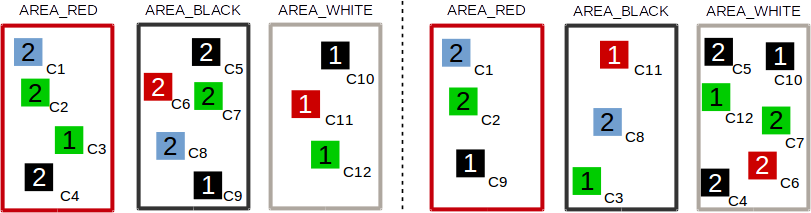
\includegraphics[scale=0.5]{figures/chapter3/case3.png}
\caption{\label{fig:case3} The initial state (left) and the goal state (right) of a task where the robot has to explain to the human partner how to move the cubes to complete the task. }
\end{figure}

%For demonstration purpose, we ran HATP with unambiguous referring expression generation calls on this setup. We are not considering the order of the cube motion in this setup. The human partner can pick and place cubes only if they have been told which one and where to place them. The robot can also pick and place cubes, but the actions are much more costly to represent the slow motion of the robot and the uncertain success. Besides, the robot can verbally communicate to the human to take a cube or to place it in an area, in these cases, the referring expression generator is used to get the cost to refer to the cube or the area respectively. Finally, the robot can also designate a cube or a place by pointing at it along with saying to take it or to place the held cube there. This pointing action has a constant cost which is higher than a simple verbal communication but lower than a complex one (with three or more relations to verbalize).

This setup has been implemented on a real PR2 robot. The architecture is similar to the one presented in Figure~\ref{fig:regarchi}, but \acrshort{hatp} has been added, and the perception has been replaced by an AR tags reader. The verbalization has been made through an ad-hoc grammar-based component, and a simple supervision has been written by Amandine Mayima to follow the plan generated by \acrshort{hatp}. Finally, a situation assessment component named TOASTER, inspired from SPARK~\cite{milliez2014framework} has been used in its simplest form, only to read AR tags from the cubes, finding if their position is inside predefined zones on the table (the area) and feeding the ontology with relevant facts. The execution of the computed plan can be found in the video available at \url{https://youtu.be/3YnGh\_t-UpY}. 

The cubes \textit{C5} and \textit{C7} are chosen to be pointed instead of verbalized. Indeed, in the world states where these cubes need to be moved, verbal referring is considered to be too costly, thus a pointing motion is preferred. For example, the cube \textit{C7} in the initial situation needs a long and complex explanation that is: \textit{``Can you take the green cube, with the number two, which is in the black storage area''} (Figure~\ref{fig:tellorpoint}). Even in the case where the pointing action takes more execution time, it could be faster for the human partner to interpret and so make the human action faster.

\begin{figure}[htb!]
\centering
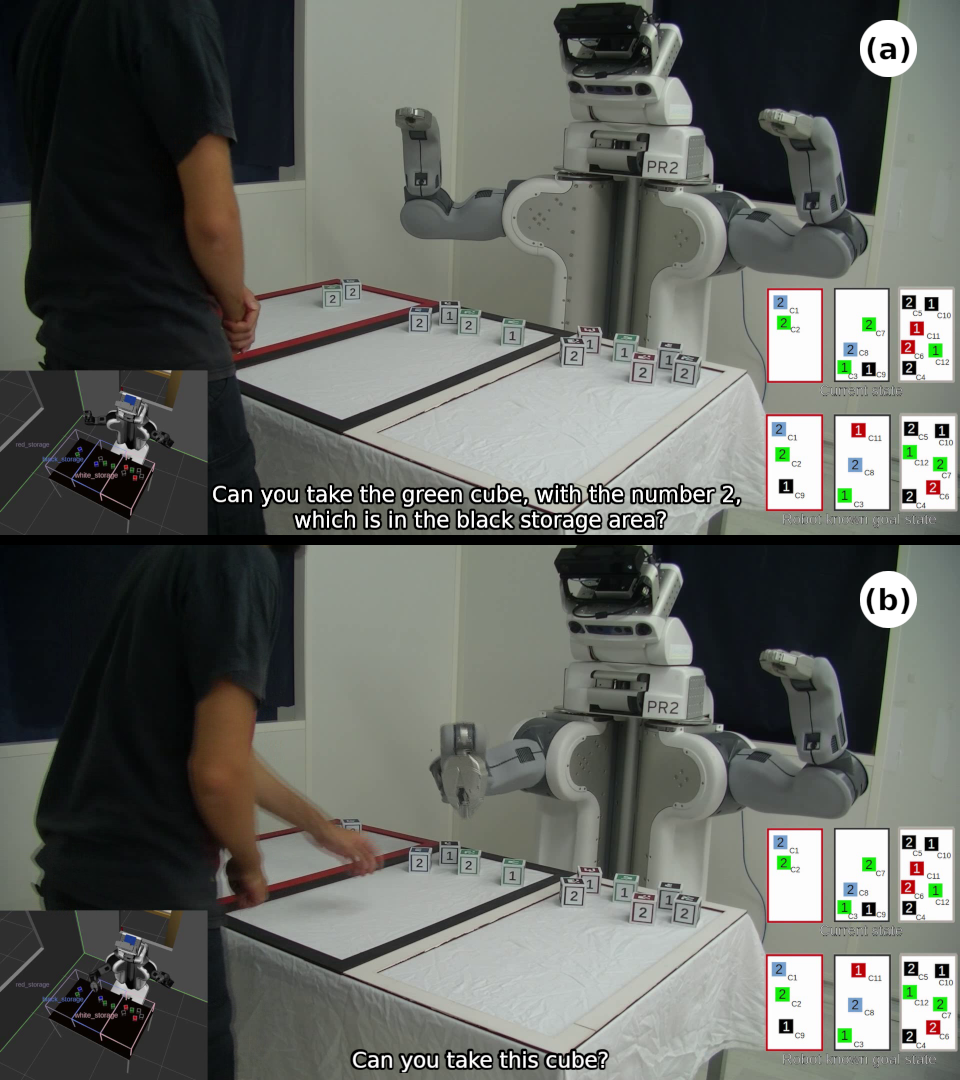
\includegraphics[width=\textwidth]{figures/chapter3/Chap3point.png}
\caption{The PR2 robot and a human sorting cubes. To designate the cube C7, the robot can either use the verbal referring (a) or point at it (b). However, the planner has found the pointing less costly for the human to understand and thus, has returned a pointing action in the executed plan (b).}
\label{fig:tellorpoint}
\end{figure}

Here, we see another benefit of our approach, it allows the planner to balance between the use of verbal communication actions, which can become complex in some states (hard to predict without a task planner), and other communication modalities. %Here, balancing was done with other means of communication, but it could also be done with other actions such as a pick and place by the robot. In the task presented here, this has no advantage, because a pick and place by the robot would be slower than an explanation or a pointing and is more likely to fail.
%Here, balancing is done with other communication mean, but can also be done other action requiring less or no communication. In our example, the robot would be slower at pick and place than explaining at or pointing to the human.
Here, verbal communication is balanced with other communication means, but it can also be balanced with other actions or assignments requiring less or no communication.



%\section{Using Past Actions in Referring Expression Generation}

\section{Conclusion}
In this chapter, we have presented an approach allowing to accurately estimate the feasibility and the cost of verbal communication actions containing referring expressions during task planning.

First, we introduced the referring expression generation problem and proposed a formalization of it dedicated to human robot interaction scenarios. Then, we presented an efficient algorithm generating referring expressions by using an ontology as a knowledge base.

Finally, we integrated this algorithm into a task planner \acrshort{hatp}, allowing it to resolve the content of such verbal communication when needed. With this extended version of \acrshort{hatp} enhanced with \acrshort{reg} capabilities, the planner can check if communication can be done in the planned world state, and it can plan different order or sequence of action depending on the communication estimation.

However, even if \acrshort{hatp} is able to maintain one belief base per agent during the planning process, it only allocates task between agents (considering the capability of each one) but does not ensure that the generated plan is known to the human nor that they have every piece of information needed to accomplish the task. Moreover, we do not take into account that the human might also plan for their own goal (which may or may not be shared with the robot). 
We propose to extend this approach by not only planning for the robot and the human, but instead planning for the robot and emulating the action, reaction and planning processes of the human the robot is interacting with.

\ifdefined\included
\else
\bibliographystyle{acm}
\bibliography{These}
\end{document}
\fi
